\documentclass[11pt,fleqn]{book} % Default font size and left-justified equations
%%----------------------------------------------------------------------------------------
%	PREAMBLE
%%----------------------------------------------------------------------------------------
%%%%%%%%%%%%%%%%%%%%%%%%%%%%%%%%%%%%%%%%%
% The Legrand Orange Book
% Structural Definitions File
% Version 2.0 (9/2/15)
%
% Original author:
% Mathias Legrand (legrand.mathias@gmail.com) with modifications by:
% Vel (vel@latextemplates.com)
% 
% This file has been downloaded from:
% http://www.LaTeXTemplates.com
%
% License:
% CC BY-NC-SA 3.0 (http://creativecommons.org/licenses/by-nc-sa/3.0/)
%
%%%%%%%%%%%%%%%%%%%%%%%%%%%%%%%%%%%%%%%%%

%%----------------------------------------------------------------------------------------
%	VARIOUS REQUIRED PACKAGES AND CONFIGURATIONS
%%----------------------------------------------------------------------------------------
\usepackage[top=3cm,bottom=3cm,left=3cm,right=3cm,headsep=10pt,a4paper]{geometry} % Page margins
\usepackage{graphicx} % Required for including pictures
\graphicspath{{Resources/Media/Pictures/}{Resources/Media/Figures/}{Resources/Media/Pictures/ChapterHeadings/}} % Specifies the directory where pictures are stored
\usepackage{lipsum} % Inserts dummy text
\usepackage{tikz} % Required for drawing custom shapes
\usepackage[english]{babel} % English language/hyphenation
\usepackage{enumitem} % Customize lists
\usepackage{dcolumn} % I ADDED
\usepackage{datatool} % I ADDED (for reading csv's)
\setlist{nolistsep} % Reduce spacing between bullet points and numbered lists
\usepackage{booktabs} % Required for nicer horizontal rules in tables
\usepackage{xcolor} % Required for specifying colors by name
%% Colors from original templates
\definecolor{ocre}{RGB}{243,102,25} % Define the orange color used for highlighting throughout the book
\definecolor{carolinablue}{RGB}{168,192,252}
%% Virginia Tech Color Palette
%  https://vt.edu/brand.html
\definecolor{VTchicagoMaroon}{RGB}{134,31,65}
\definecolor{VTburntOrange}{RGB}{232,119,34}
\definecolor{VTyardlineWhite}{RGB}{255,255,255}
\definecolor{VThokieStone}{RGB}{117,120,123}
\definecolor{VTpylonPurple}{RGB}{100,38,103}
\definecolor{VTboundlessPink}{RGB}{206,0,88}
\definecolor{VTvirginiaSunset}{RGB}{237,139,0}
\definecolor{VTtriumphantYellow}{RGB}{247,234,72}
\definecolor{VTsustainableTeal}{RGB}{80,133,144}
\definecolor{VTvibrantTurquoise}{RGB}{44,213,196}
\definecolor{VTlandgrantGrey}{RGB}{215,210,203}
\definecolor{VTskipperSmoke}{RGB}{229,225,230}
\definecolor{VTburntOrangeWEB}{RGB}{197,69,20}
\definecolor{VTcadetBlue}{RGB}{11,61,110}
% team color codes
% https://teamcolorcodes.com/virginia-tech-hokies-color-codes/
\definecolor{VTchicagoMaroonTEAM}{RGB}{106,44,62}
\definecolor{VTburntOrangeTEAM}{RGB}{207,69,32}
%%----------------------------------------------------------------------------------------
%	FONTS
%%----------------------------------------------------------------------------------------
\usepackage{draftwatermark}
\SetWatermarkText{DRAFT}
\SetWatermarkScale{1}
\usepackage{avant} % Use the Avantgarde font for headings
%\usepackage{times} % Use the Times font for headings
\usepackage{mathptmx} % Use the Adobe Times Roman as the default text font together with math symbols from the Symbol, Chancery and Computer Modern fonts
\usepackage{microtype} % Slightly tweak font spacing for aesthetics
\usepackage[utf8]{inputenc} % Required for including letters with accents
\usepackage[T1]{fontenc} % Use 8-bit encoding that has 256 glyphs
\usepackage{dirtytalk} % I ADDED
\newcommand{\RomanNumeralCaps}[1]
    {\MakeUppercase{\romannumeral #1}} % I ADDED 
%%----------------------------------------------------------------------------------------
%	BIBLIOGRAPHY AND INDEX
%%----------------------------------------------------------------------------------------
\usepackage{csquotes} % I ADDED, recommended 
\usepackage[title]{appendix} % I ADDED, for appendix labelling
\usepackage[style=numeric,citestyle=numeric,sorting=nyt,sortcites=true,autopunct=true,autolang=hyphen,hyperref=true,abbreviate=false,backend=biber]{biblatex} % I removed backref=true
\addbibresource{bibliography.bib} % BibTeX bibliography file
\defbibheading{bibempty}{}
\usepackage{calc} % For simpler calculation - used for spacing the index letter headings correctly
\usepackage{makeidx} % Required to make an index
\makeindex % Tells LaTeX to create the files required for indexing
%%----------------------------------------------------------------------------------------
%	MAIN TABLE OF CONTENTS
%%----------------------------------------------------------------------------------------
\usepackage{titletoc} % Required for manipulating the table of contents
\contentsmargin{0cm} % Removes the default margin
% Part text styling
\titlecontents{part}[0cm]
{\addvspace{20pt}\centering\large\bfseries}
{}
{}
{}
% Chapter text styling
\titlecontents{chapter}[1.25cm] % Indentation
{\addvspace{12pt}\large\sffamily\bfseries} % Spacing and font options for chapters
{\color{carolinablue!60}\contentslabel[\Large\thecontentslabel]{1.25cm}\color{carolinablue}} % Chapter number
{\color{carolinablue}}  
{\color{carolinablue!60}\normalsize\;\titlerule*[.5pc]{.}\;\thecontentspage} % Page number
% Section text styling
\titlecontents{section}[1.25cm] % Indentation
{\addvspace{3pt}\sffamily\bfseries} % Spacing and font options for sections
{\contentslabel[\thecontentslabel]{1.25cm}} % Section number
{}
{\hfill\color{black}\thecontentspage} % Page number
[]
% Subsection text styling
\titlecontents{subsection}[1.25cm] % Indentation
{\addvspace{1pt}\sffamily\small} % Spacing and font options for subsections
{\contentslabel[\thecontentslabel]{1.25cm}} % Subsection number
{}
{\ \titlerule*[.5pc]{.}\;\thecontentspage} % Page number
[]
% List of figures
\titlecontents{figure}[0em]
{\addvspace{-5pt}\sffamily}
{\thecontentslabel\hspace*{1em}}
{}
{\ \titlerule*[.5pc]{.}\;\thecontentspage}
[]
% List of tables
\titlecontents{table}[0em]
{\addvspace{-5pt}\sffamily}
{\thecontentslabel\hspace*{1em}}
{}
{\ \titlerule*[.5pc]{.}\;\thecontentspage}
[]
%#----------------------------------------------------------------------------------------
%	MINI TABLE OF CONTENTS IN PART HEADS
%#----------------------------------------------------------------------------------------
% Chapter text styling
\titlecontents{lchapter}[-7em] % Indenting
{\addvspace{15pt}\large\sffamily\bfseries} % Spacing and font options for chapters
{\color{carolinablue}\contentslabel[\Large\thecontentslabel]{1.25cm}\color{carolinablue}} % Chapter number
{}  
{\color{carolinablue}\normalsize\sffamily\bfseries\titlerule*[1pc]{.}\thecontentspage} % Page number
% Section text styling
\titlecontents{lsection}[-7em] % Indenting
{\sffamily\small} % Spacing and font options for sections
{\contentslabel[\thecontentslabel]{1.25cm}} % Section number
{}
{}
% Subsection text styling
\titlecontents{lsubsection}[.5em] % Indentation
{\normalfont\footnotesize\sffamily} % Font settings
{}
{}
{}
%%----------------------------------------------------------------------------------------
%	PAGE HEADERS
%%----------------------------------------------------------------------------------------
\usepackage{fancyhdr} % Required for header and footer configuration
\pagestyle{fancy}
\renewcommand{\chaptermark}[1]{\markboth{\sffamily\normalsize\bfseries\chaptername\ \thechapter.\ #1}{}} % Chapter text font settings
\renewcommand{\sectionmark}[1]{\markright{\sffamily\normalsize\thesection\hspace{5pt}#1}{}} % Section text font settings
\fancyhf{} \fancyhead[LE,RO]{\sffamily\normalsize\thepage} % Font setting for the page number in the header
\fancyhead[LO]{\rightmark} % Print the nearest section name on the left side of odd pages
\fancyhead[RE]{\leftmark} % Print the current chapter name on the right side of even pages
\renewcommand{\headrulewidth}{0.5pt} % Width of the rule under the header
\addtolength{\headheight}{2.5pt} % Increase the spacing around the header slightly
\renewcommand{\footrulewidth}{0pt} % Removes the rule in the footer
\fancypagestyle{plain}{\fancyhead{}\renewcommand{\headrulewidth}{0pt}} % Style for when a plain pagestyle is specified
% Removes the header from odd empty pages at the end of chapters
\makeatletter
\renewcommand{\cleardoublepage}{
%\clearpage\ifodd\c@page\else % I COMMENTED OUT
\hbox{}
\vspace*{\fill}
\thispagestyle{empty}
\newpage
%\fi % I COMMENTED OUT
}
%%----------------------------------------------------------------------------------------
%	THEOREM STYLES
%%----------------------------------------------------------------------------------------
\usepackage{amsmath,amsfonts,amssymb,amsthm} % For math equations, theorems, symbols, etc
\newcommand{\intoo}[2]{\mathopen{]}#1\,;#2\mathclose{[}}
\newcommand{\ud}{\mathop{\mathrm{{}d}}\mathopen{}}
\newcommand{\intff}[2]{\mathopen{[}#1\,;#2\mathclose{]}}
\newtheorem{notation}{Notation}[chapter]
% Boxed/framed environments
\newtheoremstyle{carolinabluenumbox}% % Theorem style name
{0pt}% Space above
{0pt}% Space below
{\normalfont}% % Body font
{}% Indent amount
{\small\bf\sffamily\color{carolinablue}}% % Theorem head font
{\;}% Punctuation after theorem head
{0.25em}% Space after theorem head
{\small\sffamily\color{carolinablue}\thmname{#1}\nobreakspace\thmnumber{\@ifnotempty{#1}{}\@upn{#2}}% Theorem text (e.g. Theorem 2.1)
\thmnote{\nobreakspace\the\thm@notefont\sffamily\bfseries\color{black}---\nobreakspace#3.}} % Optional theorem note
\renewcommand{\qedsymbol}{$\blacksquare$}% Optional qed square
\newtheoremstyle{blacknumex}% Theorem style name
{5pt}% Space above
{5pt}% Space below
{\normalfont}% Body font
{} % Indent amount
{\small\bf\sffamily}% Theorem head font
{\;}% Punctuation after theorem head
{0.25em}% Space after theorem head
{\small\sffamily{\tiny\ensuremath{\blacksquare}}\nobreakspace\thmname{#1}\nobreakspace\thmnumber{\@ifnotempty{#1}{}\@upn{#2}}% Theorem text (e.g. Theorem 2.1)
\thmnote{\nobreakspace\the\thm@notefont\sffamily\bfseries---\nobreakspace#3.}}% Optional theorem note
\newtheoremstyle{blacknumbox} % Theorem style name
{0pt}% Space above
{0pt}% Space below
{\normalfont}% Body font
{}% Indent amount
{\small\bf\sffamily}% Theorem head font
{\;}% Punctuation after theorem head
{0.25em}% Space after theorem head
{\small\sffamily\thmname{#1}\nobreakspace\thmnumber{\@ifnotempty{#1}{}\@upn{#2}}% Theorem text (e.g. Theorem 2.1)
\thmnote{\nobreakspace\the\thm@notefont\sffamily\bfseries---\nobreakspace#3.}}% Optional theorem note
% Non-boxed/non-framed environments
\newtheoremstyle{carolinabluenum}% % Theorem style name
{5pt}% Space above
{5pt}% Space below
{\normalfont}% % Body font
{}% Indent amount
{\small\bf\sffamily\color{carolinablue}}% % Theorem head font
{\;}% Punctuation after theorem head
{0.25em}% Space after theorem head
{\small\sffamily\color{carolinablue}\thmname{#1}\nobreakspace\thmnumber{\@ifnotempty{#1}{}\@upn{#2}}% Theorem text (e.g. Theorem 2.1)
\thmnote{\nobreakspace\the\thm@notefont\sffamily\bfseries\color{black}---\nobreakspace#3.}} % Optional theorem note
\renewcommand{\qedsymbol}{$\blacksquare$}% Optional qed square
\makeatother
% Defines the theorem text style for each type of theorem to one of the three styles above
\newcounter{dummy} 
\numberwithin{dummy}{section}
\theoremstyle{carolinabluenumbox}
\newtheorem{theoremeT}[dummy]{Theorem}
\newtheorem{problem}{Problem}[chapter]
%%%
%% For organizing PQE's and their solutions (I added) 
% allows separate publication, even with problem and solution together in text
% http://ctan.math.washington.edu/tex-archive/macros/latex/contrib/exsol/exsol.pdf
%\def\solutionname{Solution \thechapter.\arabic{exercise}} % failed
\usepackage[copyexercisesinsolutions]{exsol}
\renewcommand{\exercisesname}{Problems, Questions, and Exercises for Chapter \thechapter}
\renewcommand{\exercisename}{Problem}
\renewcommand{\theexercise}{\thechapter.\arabic{exercise}}
%\renewcommand{\solutionname}{Solution \thechapter.\arabic{exercise}} % failed
%\renewcommand*\solutionname{Solution \thechapter.\arabic{exercise}} % failed
%\def\solutionname{Solution \thechapter.\arabic{exercise}} % failed
% above is my formatting of exsol
\newtheorem{exerciseT}{Exercise}[chapter]
\theoremstyle{blacknumex}
\newtheorem{exampleT}{Example}[chapter]
\theoremstyle{blacknumbox}
\newtheorem{vocabulary}{Vocabulary}[chapter]
\newtheorem{definitionT}{Definition}[section]
\newtheorem{corollaryT}[dummy]{Corollary}
\theoremstyle{carolinabluenum}
\newtheorem{proposition}[dummy]{Proposition}
%%----------------------------------------------------------------------------------------
%	DEFINITION OF COLORED BOXES
%%----------------------------------------------------------------------------------------
\RequirePackage[framemethod=default]{mdframed} % Required for creating the theorem, definition, exercise and corollary boxes
% Theorem box
\newmdenv[skipabove=7pt,
skipbelow=7pt,
backgroundcolor=black!5,
linecolor=carolinablue,
innerleftmargin=5pt,
innerrightmargin=5pt,
innertopmargin=5pt,
leftmargin=0cm,
rightmargin=0cm,
innerbottommargin=5pt]{tBox}
% Exercise box	  
\newmdenv[skipabove=7pt,
skipbelow=7pt,
rightline=false,
leftline=true,
topline=false,
bottomline=false,
backgroundcolor=carolinablue!10,
linecolor=carolinablue,
innerleftmargin=5pt,
innerrightmargin=5pt,
innertopmargin=5pt,
innerbottommargin=5pt,
leftmargin=0cm,
rightmargin=0cm,
linewidth=4pt]{eBox}	
% Definition box
\newmdenv[skipabove=7pt,
skipbelow=7pt,
rightline=false,
leftline=true,
topline=false,
bottomline=false,
linecolor=carolinablue,
innerleftmargin=5pt,
innerrightmargin=5pt,
innertopmargin=0pt,
leftmargin=0cm,
rightmargin=0cm,
linewidth=4pt,
innerbottommargin=0pt]{dBox}	
% Corollary box
\newmdenv[skipabove=7pt,
skipbelow=7pt,
rightline=false,
leftline=true,
topline=false,
bottomline=false,
linecolor=gray,
backgroundcolor=black!5,
innerleftmargin=5pt,
innerrightmargin=5pt,
innertopmargin=5pt,
leftmargin=0cm,
rightmargin=0cm,
linewidth=4pt,
innerbottommargin=5pt]{cBox}
% Creates an environment for each type of theorem and assigns it a theorem text style from the "Theorem Styles" section above and a colored box from above
\newenvironment{theorem}{\begin{tBox}\begin{theoremeT}}{\end{theoremeT}\end{tBox}}
% (I added) exercise -> exercise_original
\newenvironment{exercise_original}{\begin{eBox}\begin{exerciseT}}{\hfill{\color{carolinablue}\tiny\ensuremath{\blacksquare}}\end{exerciseT}\end{eBox}}				  
\newenvironment{definition}{\begin{dBox}\begin{definitionT}}{\end{definitionT}\end{dBox}}	
\newenvironment{example}{\begin{exampleT}}{\hfill{\tiny\ensuremath{\blacksquare}}\end{exampleT}}		
\newenvironment{corollary}{\begin{cBox}\begin{corollaryT}}{\end{corollaryT}\end{cBox}}	
%%----------------------------------------------------------------------------------------
%	REMARK ENVIRONMENT
%%----------------------------------------------------------------------------------------
\newenvironment{remark}{\par\vspace{10pt}\small % Vertical white space above the remark and smaller font size
\begin{list}{}{
\leftmargin=35pt % Indentation on the left
\rightmargin=25pt}\item\ignorespaces % Indentation on the right
\makebox[-2.5pt]{\begin{tikzpicture}[overlay]
\node[draw=carolinablue!60,line width=1pt,circle,fill=carolinablue!25,font=\sffamily\bfseries,inner sep=2pt,outer sep=0pt] at (-15pt,0pt){\textcolor{carolinablue}{R}};\end{tikzpicture}} % Orange R in a circle
\advance\baselineskip -1pt}{\end{list}\vskip5pt} % Tighter line spacing and white space after remark
%%----------------------------------------------------------------------------------------
%	SECTION NUMBERING IN THE MARGIN
%%----------------------------------------------------------------------------------------
\makeatletter
\renewcommand{\@seccntformat}[1]{\llap{\textcolor{carolinablue}{\csname the#1\endcsname}\hspace{1em}}}                    
\renewcommand{\section}{\@startsection{section}{1}{\z@}
{-4ex \@plus -1ex \@minus -.4ex}
{1ex \@plus.2ex }
{\normalfont\large\sffamily\bfseries}}
\renewcommand{\subsection}{\@startsection {subsection}{2}{\z@}
{-3ex \@plus -0.1ex \@minus -.4ex}
{0.5ex \@plus.2ex }
{\normalfont\sffamily\bfseries}}
\renewcommand{\subsubsection}{\@startsection {subsubsection}{3}{\z@}
{-2ex \@plus -0.1ex \@minus -.2ex}
{.2ex \@plus.2ex }
{\normalfont\small\sffamily\bfseries}}                        
\renewcommand\paragraph{\@startsection{paragraph}{4}{\z@}
{-2ex \@plus-.2ex \@minus .2ex}
{.1ex}
{\normalfont\small\sffamily\bfseries}}
%%----------------------------------------------------------------------------------------
%	PART HEADINGS
%%----------------------------------------------------------------------------------------
% numbered part in the table of contents
\newcommand{\@mypartnumtocformat}[2]{%
\setlength\fboxsep{0pt}%
\noindent\colorbox{carolinablue!20}{\strut\parbox[c][.7cm]{\ecart}{\color{carolinablue!70}\Large\sffamily\bfseries\centering#1}}\hskip\esp\colorbox{carolinablue!40}{\strut\parbox[c][.7cm]{\linewidth-\ecart-\esp}{\Large\sffamily\centering#2}}}%
%%%%%%%%%%%%%%%%%%%%%%%%%%%%%%%%%%
% unnumbered part in the table of contents
\newcommand{\@myparttocformat}[1]{%
\setlength\fboxsep{0pt}%
\noindent\colorbox{carolinablue!40}{\strut\parbox[c][.7cm]{\linewidth}{\Large\sffamily\centering#1}}}%
%%%%%%%%%%%%%%%%%%%%%%%%%%%%%%%%%%
\newlength\esp
\setlength\esp{4pt}
\newlength\ecart
\setlength\ecart{1.2cm-\esp}
\newcommand{\thepartimage}{}%
\newcommand{\partimage}[1]{\renewcommand{\thepartimage}{#1}}%
\def\@part[#1]#2{%
\ifnum \c@secnumdepth >-2\relax%
\refstepcounter{part}%
\addcontentsline{toc}{part}{\texorpdfstring{\protect\@mypartnumtocformat{\thepart}{#1}}{\partname~\thepart\ ---\ #1}}
\else%
\addcontentsline{toc}{part}{\texorpdfstring{\protect\@myparttocformat{#1}}{#1}}%
\fi%
\startcontents%
\markboth{}{}%
{\thispagestyle{empty}%
\begin{tikzpicture}[remember picture,overlay]%
\node at (current page.north west){\begin{tikzpicture}[remember picture,overlay]%	
\fill[carolinablue!20](0cm,0cm) rectangle (\paperwidth,-\paperheight);
\node[anchor=north] at (4cm,-3.25cm){\color{carolinablue!40}\fontsize{220}{100}\sffamily\bfseries\thepart}; 
\node[anchor=south east] at (\paperwidth-1cm,-\paperheight+1cm){\parbox[t][][t]{8.5cm}{
\printcontents{l}{0}{\setcounter{tocdepth}{1}}%
}};
\node[anchor=north east] at (\paperwidth-1.5cm,-3.25cm){\parbox[t][][t]{15cm}{\strut\raggedleft\color{white}\fontsize{30}{30}\sffamily\bfseries#2}};
\end{tikzpicture}};
\end{tikzpicture}}%
\@endpart}
\def\@spart#1{%
\startcontents%
\phantomsection
{\thispagestyle{empty}%
\begin{tikzpicture}[remember picture,overlay]%
\node at (current page.north west){\begin{tikzpicture}[remember picture,overlay]%	
\fill[carolinablue!20](0cm,0cm) rectangle (\paperwidth,-\paperheight);
\node[anchor=north east] at (\paperwidth-1.5cm,-3.25cm){\parbox[t][][t]{15cm}{\strut\raggedleft\color{white}\fontsize{30}{30}\sffamily\bfseries#1}};
\end{tikzpicture}};
\end{tikzpicture}}
\addcontentsline{toc}{part}{\texorpdfstring{%
\setlength\fboxsep{0pt}%
\noindent\protect\colorbox{carolinablue!40}{\strut\protect\parbox[c][.7cm]{\linewidth}{\Large\sffamily\protect\centering #1\quad\mbox{}}}}{#1}}%
\@endpart}
\def\@endpart{\vfil\newpage
\if@twoside
\if@openright
\null
%% I COMMENTED OUT 2 LINES BELOW
%\thispagestyle{empty}%
%\newpage
\fi
\fi
\if@tempswa
\twocolumn
\fi}
%%----------------------------------------------------------------------------------------
%	CHAPTER HEADINGS
%%----------------------------------------------------------------------------------------
% A switch to conditionally include a picture, implemented by  Christian Hupfer
\newif\ifusechapterimage
\usechapterimagetrue
\newcommand{\thechapterimage}{}%
\newcommand{\chapterimage}[1]{\ifusechapterimage\renewcommand{\thechapterimage}{#1}\fi}%
\newcommand{\autodot}{.}
\def\@makechapterhead#1{%
{\parindent \z@ \raggedright \normalfont
\ifnum \c@secnumdepth >\m@ne
\if@mainmatter
\begin{tikzpicture}[remember picture,overlay]
\node at (current page.north west)
{\begin{tikzpicture}[remember picture,overlay]
\node[anchor=north west,inner sep=0pt] at (0,0) {\ifusechapterimage\includegraphics[width=\paperwidth]{\thechapterimage}\fi};
\draw[anchor=west] (\Gm@lmargin,-9cm) node [line width=2pt,rounded corners=15pt,draw=VThokieStone,fill=white,fill opacity=0.8,inner sep=15pt]{\strut\makebox[22cm]{}};
\draw[anchor=west] (\Gm@lmargin+.3cm,-9cm) node {\huge\sffamily\bfseries\color{black}\thechapter\autodot~#1\strut};
\end{tikzpicture}};
\end{tikzpicture}
\else
\begin{tikzpicture}[remember picture,overlay]
\node at (current page.north west)
{\begin{tikzpicture}[remember picture,overlay]
\node[anchor=north west,inner sep=0pt] at (0,0) {\ifusechapterimage\includegraphics[width=\paperwidth]{\thechapterimage}\fi};
\draw[anchor=west] (\Gm@lmargin,-9cm) node [line width=2pt,rounded corners=15pt,draw=VThokieStone,fill=white,fill opacity=0.8,inner sep=15pt]{\strut\makebox[22cm]{}};
\draw[anchor=west] (\Gm@lmargin+.3cm,-9cm) node {\huge\sffamily\bfseries\color{black}#1\strut};
\end{tikzpicture}};
\end{tikzpicture}
\fi\fi\par\vspace*{270\p@}}}
%-------------------------------------------
\def\@makeschapterhead#1{%
\begin{tikzpicture}[remember picture,overlay]
\node at (current page.north west)
{\begin{tikzpicture}[remember picture,overlay]
\node[anchor=north west,inner sep=0pt] at (0,0) {\ifusechapterimage\includegraphics[width=\paperwidth]{\thechapterimage}\fi};
\draw[anchor=west] (\Gm@lmargin,-9cm) node [line width=2pt,rounded corners=15pt,draw=VThokieStone,fill=white,fill opacity=0.8,inner sep=15pt]{\strut\makebox[22cm]{}};
\draw[anchor=west] (\Gm@lmargin+.3cm,-9cm) node {\huge\sffamily\bfseries\color{black}#1\strut};
\end{tikzpicture}};
\end{tikzpicture}
\par\vspace*{270\p@}}
\makeatother
%%----------------------------------------------------------------------------------------
%	HYPERLINKS IN THE DOCUMENTS
%%----------------------------------------------------------------------------------------
% to create automatic labels for sections, since there are too many
% to reference sections, use \Cref{sec:"SECTION TITLE"} without quotes
% gets applied to chapters too ?
%\usepackage{etoolbox}
%\makeatletter
%\patchcmd{\@sect}% <cmd>
%  {\@xsect}% <search>
%  {\label{sec:#8}\@xsect}% <replace>
%  {}{}% <successs><failure>
%\makeatother
% from Thesis package
% links for references
%\RequirePackage[final,colorlinks=true,allcolors=blue]{hyperref}
% removed backref=true,pagebackref=true
\usepackage[final,hidelinks,hyperindex=true,colorlinks=false,breaklinks=true,urlcolor=carolinablue,bookmarks=true,bookmarksopen=false,pdftitle={Title},pdfauthor={Author}]{hyperref}
\usepackage[nameinlink,noabbrev]{cleveref}
%\usepackage{autonum} % I COMMENTED, incompatible package with biblatex
\usepackage{xr} % I ADDED, to reference labels from main document from Solution Manual
\usepackage{bookmark}
\bookmarksetup{
open,
numbered,
addtohook={%
\ifnum\bookmarkget{level}=0 % chapter
\bookmarksetup{bold}%
\fi
\ifnum\bookmarkget{level}=-1 % part
\bookmarksetup{color=carolinablue,bold}%
\fi
}
} % importing packages and defining settings, environments, and commands
%%%%%
%%  below block to reference main document labels from Solution Manual
% may be duplicating labels?  (getting warnings, not sure if affecting behavior)
\makeatletter
\newcommand*{\addFileDependency}[1]{% argument=file name and extension
  \typeout{(#1)}
  \@addtofilelist{#1}
  \IfFileExists{#1}{}{\typeout{No file #1.}}
}
\makeatother

\newcommand*{\myexternaldocument}[1]{%
    \externaldocument{#1}%
    \addFileDependency{#1.tex}%
    \addFileDependency{#1.aux}%
}
%%%%%
\myexternaldocument{mainBook}
\begin{document}
%%----------------------------------------------------------------------------------------
%	TITLE PAGE
%%----------------------------------------------------------------------------------------
\begingroup
\thispagestyle{empty}
\begin{tikzpicture}[remember picture,overlay]
\node[inner sep=0pt] (background) at (current page.center) {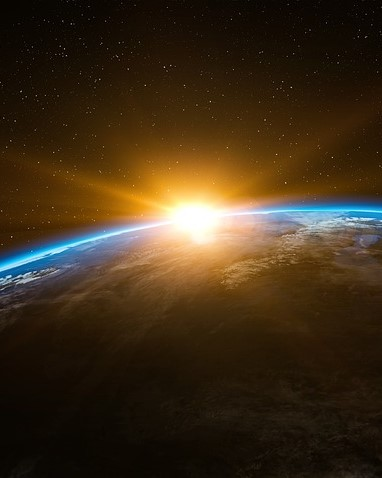
\includegraphics[width=\paperwidth,height=\paperheight]{space2}}; % original picture size was 8.08"x11.56"
\draw (current page.south) node [fill=white!30!white,fill opacity=0.6,text opacity=1,inner sep=1cm, anchor=south]{\Huge\centering\bfseries\sffamily\parbox[c][][t]{\paperwidth}{\centering \textsc{Systems Thinking, Engineering, and Analysis}\\[21pt] % Book title
{\huge Solution Manual}}}; % Author name
\end{tikzpicture}
\vfill
\endgroup
%%----------------------------------------------------------------------------------------
%	COPYRIGHT PAGE
%%----------------------------------------------------------------------------------------
\newpage
~\vfill
\thispagestyle{empty}
\noindent Copyright \copyright\ 2018 Wolter J Fabrycky\\ % Copyright notice
\noindent \textsc{Published by ACE, a Zachary D Miller company}\\ % Publisher
\noindent \textsc{\url{www.a2i2.com}}\\ % URL
\noindent Licensed under the Creative Commons Attribution-NonCommercial 3.0 Unported License (the ``License''). You may not use this file except in compliance with the License. You may obtain a copy of the License at \url{http://creativecommons.org/licenses/by-nc/3.0}. Unless required by applicable law or agreed to in writing, software distributed under the License is distributed on an \textsc{``as is'' basis, without warranties or conditions of any kind}, either express or implied. See the License for the specific language governing permissions and limitations under the License.\\ % License information
\noindent \textit{First electronic publication, 2018} % Printing/edition date
%%----------------------------------------------------------------------------------------
%	TABLE OF CONTENTS
%%----------------------------------------------------------------------------------------
%\usechapterimagefalse % If you don't want to include a chapter image, use this to toggle images off - it can be enabled later with \usechapterimagetrue
\chapterimage{chain.jpg} % Table of contents heading image
\pagestyle{empty} % No headers
\tableofcontents % Print the table of contents itself
% undesirable as an e-book
%\cleardoublepage % Forces the first chapter to start on an odd page so it's on the right
\pagestyle{fancy} % Print headers again
\begin{exsol@exercise}{1.1}
    \label{sea-1-26}
        Describe how systems thinking differs from systems engineering.
\end{exsol@exercise}
\begin{exsol@solution}{}
        Human society is characterized by its culture. Each human culture manifests itself through the medium of technology. It takes more than a single step for society to transition from the past, to present and future technology states. A common societal response is often to make the transition and then to adopt a static pattern of behavior. A better response would be to continuously seek new but well-thought-out possibilities for advancement. Improvement in technological literacy embracing systems thinking should increase the population of individuals capable of participating in this desirable endeavor. \textbf{Reference:}
\end{exsol@solution}
\begin{exsol@exercise}{1.2}
    \label{sea-1-1}
        For a system with which you are familiar, justify why it is a system according to the definition in \Cref{sec:sectorsComprisingWorld}.
\end{exsol@exercise}
\begin{exsol@solution}{}
        A river system (Mississippi) is an assemblage of a watershed, tributaries, and river banks that conveys water from the continental U.S. to the Gulf of Mexico. A municipal transportation system (Chicago) is an assemblage of trains, buses, subways, etc. that transports people among many city locations. A system of organization and management (Matrix) is based on a morphology and procedure, coordinating both line and support functions. An automobile manufacturer is a combination of factories, organizations, dealerships, etc., that delivers automobiles and related support services. A home is an assemblage of land, structure, utilities, furnishings, and people that provides a supportive place to live for one or more families. \textbf{Reference:}
\end{exsol@solution}
\begin{exsol@exercise}{1.3}
    \label{sea-1-2}
        Describe the components, attributes, and relationships in the system you used in Problem \ref{sea-1-1}.
\end{exsol@exercise}
\begin{exsol@solution}{}
        The major components of a home are listed in Answer 1 above. Attributes include acreage, terrain, square footage, utility capacities, styles of decorating and furnishing, personalities, and philosophies. Relationships include layout, allocation of space to people, and approaches to living together. \textbf{Reference:}
\end{exsol@solution}
\begin{exsol@exercise}{1.4}
    \label{sea-1-3}
        Name any system which includes a material that transforms over the system's life cycle and identify its structural components, operating components, and flow components.
\end{exsol@exercise}
\begin{exsol@solution}{}
        A chemica1 processing plant is composed of structural components (building, tanks, piping), operating components (pumps, valves, controls), and flow components (chemical constituents, energy, information). \textbf{Reference:}
\end{exsol@solution}
\begin{exsol@exercise}{1.5}
    \label{sea-1-4_5}
        Name any complex system and
        \begin{enumerate}[label=\alph*)]
            \item Define the hierarchy related to the system.
            \item Define the system boundaries.
        \end{enumerate}
\end{exsol@exercise}
\begin{exsol@solution}{}
        A dam system can be considered a complex system.
        \begin{enumerate}[label=\alph*)]
            \item todo
            \item The boundaries of a dam system can be limited to the physical dam. Alternatively, the human-modified river system, which now has a lake, can be considered a part of the dam system. The related road system, for which the dam now provides a bridge over the river, can be included. The region’s tourism service system, for which the dam system now provides an array of additional services, can be included. \textbf{Reference:}
        \end{enumerate}
\end{exsol@solution}
\begin{exsol@exercise}{1.6}
    \label{sea-1-6_7_8}
        Identify and contrast
        \begin{enumerate}[label=\alph*)]
            \item Physical versus conceptual systems.
            \item Static versus dynamic systems.
            \item Closed versus open systems.
        \end{enumerate}
\end{exsol@exercise}
\begin{exsol@solution}{}
        \begin{enumerate}[label=\alph*)]
            \item A physical system such as a watershed has components which manifest themselves in space and time, whereas a conceptual system such as a work breakdown structure has no physical manifestations. It is only a plan for action. Reference: Section 1.2.2 (pages 6-7).
            \item A static system such as a highway system may be contrasted with an airline system, which is a dynamic system. In the former, structure exists without activity whereas in the latter, structural components are combined with the activities of aircraft being loaded and unloaded, aircraft in flight, and controls which govern the entire operation. Reference: Section 1.2.3 (page 7).
            \item A cannon is an example of a closed system. When a cannon is fired, a one–to–one correspondence exists between the initial and final states. However, the defense contractor’s design and manufacturing organization that produced the cannon and associated projectile is an open system, with a dynamic interaction of system components. These system components must be reconfigured and adapted to cope with changing requirements. \textbf{Reference:}
        \end{enumerate}
\end{exsol@solution}
\begin{exsol@exercise}{1.7}
    \label{sea-1-15}
        For any system of the following types, name any system property
        \begin{enumerate}[label=\alph*)]
            \item Dynamic system.
            \item Steady-state system.
        \end{enumerate}
\end{exsol@exercise}
\begin{exsol@solution}{}
        \textbf{Reference:}
\end{exsol@solution}
\begin{exsol@exercise}{1.8}
    \label{sea-1-9}
        For each of the following systems, define a unique system and describe it in terms of components, attributes, and relationships
        \begin{enumerate}[label=\alph*)]
            \item Natural system.
            \item Human-made system.
            \item Human-modified system.
        \end{enumerate}
\end{exsol@exercise}
\begin{exsol@solution}{}
        \begin{enumerate}[label=\alph*)]
            \item A watershed is a natural system made up of objects or components such as land, vegetation, and the watercourse; attributes such as the soil type, timber species, and the river width; and relationships such as the distribution of the attributes over the terrain.
            \item A chemical processing plant is a human–made system with components described in Answer 3 above, attributes such as tank volume and pipe diameter, and relationships such as the flow rates and the yield of final product per energy unit utilized.
            \item A person with a pacemaker is a human-modified system with components of body parts and pacemaker parts, attributes such as body mass, diseases, attitudes, battery, controller, and electrodes, and relationships such as implantation location, rhythm, and signal strength. \textbf{Reference:}
        \end{enumerate}
\end{exsol@solution}
\begin{exsol@exercise}{1.9}
    \label{sea-1-10_11_12}
        For any Human-made system (including the system from \Cref{sea-1-9})
        \begin{enumerate}[label=\alph*)]
            \item Identify the system's purpose(s) and potential metrics to present its value.
            \item Describe the system's state at any arbitrary time during operation, at least one system behavior, and an overview of the system's process.
            \item Name any two related components of the system, define the purpose of each component as it relates to the other, and the necessary attributes of the component pair such that they contribute to the purpose(s) of the entire system.
        \end{enumerate}
\end{exsol@exercise}
\begin{exsol@solution}{}
        \begin{enumerate}[label=\alph*)]
            \item The purposes of a chemical processing plant in a market economy are to produce one or more chemical products and possibly byproducts that can be sold at a profit while fulfilling obligations to stakeholders and the public. Measures of worth include production cost per unit volume, product quality, flexibility of product mix, benefits to stakeholders, and compatibility with society. \textbf{Reference:}
            \item During startup the state of a chemical processing plant is that pipes and vessels are filled to a certain location and empty after that location; pumps for vessels being filled are running and valves are open while other pumps are not running and valves are closed. A behavior is that when a vessel is filled, the control system turns off the pump (in a batch system) or reduces its speed (in a continuous system) and activates the next step in the process. The process is to start up, achieve the designated operational speed for each subsystem, continuously monitor the production results and make needed adjustments, and eventually shut down and clean out. \textbf{Reference:}
            \item A pump and the tank it fills have a relationship. The pump provides the material that the tank needs, while the tank provides a location where the pump can store the material it needs to deliver. The attributes of the pump must be engineered so that it can reliably move the material(s) the tank needs at an adequate rate for any given speed of overall system operation. The attributes of the tank must be engineered so that it can store the quantities of material the pump must deliver without corrosion or contamination. Thus the downstream components have the material they need to fulfill the plant’s production purpose without problems of quality or pollution. \textbf{Reference:}
        \end{enumerate}
\end{exsol@solution}
\begin{exsol@exercise}{1.10}
    \label{sea-1-14}
        For any Human-modified system (including the system from \Cref{sea-1-9}), name some positive and negative impact(s) of the modification to the natural system.
\end{exsol@exercise}
\begin{exsol@solution}{}
        Human introduction of plant or animal species into regions where they do not naturally occur can provide the benefits of those species in the new regions, but the new species may become excessively dominant in those regions due to lack of natural enemies, crowding out or harming beneficial native species. \textbf{Reference:}
\end{exsol@solution}
\begin{exsol@exercise}{1.11}
    \label{sea-1-13}
        Give examples of each of the following
        \begin{enumerate}[label=\alph*)]
            \item First-order relationship.
            \item Second-order relationship.
            \item Redundance.
        \end{enumerate}
\end{exsol@exercise}
\begin{exsol@solution}{}
        \begin{enumerate}[label=\alph*)]
            \item In a computer system, the power supply and system board have a first-order relationship because the system board must receive the reduced voltage produced by the power supply in order to function, and the power supply would be useless if there were no system board to perform and coordinate the computer functions.
            \item The system board has a second-order relationship with a math coprocessor, or a video processor, or with video memory. The system board could perform the functions of these additional components, but the added components relieve the system board’s workload, thereby improving its performance.
            \item  A second power supply or a mirror image hard disk drive provide redundance, ensuring that the system board can continue receiving electrical power and the data storage function, thereby helping to assure continuation of the computer system function. \textbf{Reference:}
        \end{enumerate}
\end{exsol@solution}
\begin{exsol@exercise}{1.12}
    \label{sea-1-16}
        Name any system that operates at equilibrium and another system that degrades over time.
\end{exsol@exercise}
\begin{exsol@solution}{}
        A forest reaches equilibrium. A tree is in equilibrium until it dies, and then it disintegrates. \textbf{Reference:}
\end{exsol@solution}
\begin{exsol@exercise}{1.13}
    \label{sea-1-17}
        The United States government, for example, can be divided and described as three individual entities of the executive, legislative, and judicial branches. Create an argument for why a government of this structure should either be considered a single system or three systems.
\end{exsol@exercise}
\begin{exsol@solution}{}
        The government described is a single system because the branches thereof are functionally related. \textbf{Reference:}
\end{exsol@solution}
\begin{exsol@exercise}{1.14}
    \label{sea-1-19}
        Give any example of cybernetics and define why the example is appropriate.
\end{exsol@exercise}
\begin{exsol@solution}{}
        Cybernetics may be described and explained by considering the early mechanical version of a governor to control the revolutions per minute (RPM) of an engine. Centrifugal force, acting through a weight mechanism on the flywheel, is used to sense RPM. The outward movement of the weight against a spring acts through a link to decrease the throttle setting, thus reducing engine speed. \textbf{Reference:}
\end{exsol@solution}
\begin{exsol@exercise}{1.15}
    \label{sea-1-21}
        Do all systems at higher levels of Boulding's Hierarchy necessarily incorporate the lower levels of the hierarchy? If not, provide a specific system example.
\end{exsol@exercise}
\begin{exsol@solution}{}
        \textbf{Reference:}
\end{exsol@solution}
\begin{exsol@exercise}{1.16}
    \label{sea-1-22}
        Describe a novel system that may be necessary for society 50 to 100 years in the future and
        \begin{enumerate}[label=\alph*)]
            \item Define the system requirements.
            \item Define the system objectives.
        \end{enumerate}
\end{exsol@exercise}
\begin{exsol@solution}{}
        Efficient transportation system to the Moon and/or Mars. \textbf{Reference:}
\end{exsol@solution}
\begin{exsol@exercise}{1.17}
    \label{sea-1-25}
        For the system described in Question \ref{sea-1-22}
        \begin{enumerate}[label=\alph*)]
            \item Identify factors which led to the need for a new system.
            \item Identify other societal factors which may evolve in parallel and lead to other changes or innovations.
        \end{enumerate}
\end{exsol@exercise}
\begin{exsol@solution}{}
        \begin{enumerate}[label=\alph*)]
            \item Factors driving technological change include attempts to respond to unmet current needs and attempts to perform ongoing activities in a more efficient and effective manner, as well as social factors, political objectives, ecological concerns, and the desire for environmental sustainability. \textbf{Reference:}
            \item todo
        \end{enumerate}
\end{exsol@solution}
\begin{exsol@exercise}{1.18}
    \label{sea-1-23}
        Compare and contrast systemology and synthesis.
\end{exsol@exercise}
\begin{exsol@solution}{}
        Both systemology and synthesis produce systems. Systemology produces a system of processes by which systems are brought into being and carried through the life cycle. Synthesis produces any kind of system. Synthesis is a part of systemology and also a product of systemology. \textbf{Reference:}
\end{exsol@solution}
\begin{exsol@exercise}{1.19}
    \label{sea-1-24}
        Classify a technical system.
\end{exsol@exercise}
\begin{exsol@solution}{}
        The phrase “technical system” is used to represent all types of human–made artifacts, including engineered products and processes. Classifying a technical system is generally difficult, because a technical system derives its inputs from several disciplines or fields which may be very different from one another. \textbf{Reference:}
\end{exsol@solution}
\begin{exsol@exercise}{1.20}
    \label{sea-1-27}
        Compare and contrast the attributes of the Machine (Industrial) Age and the Systems Age.
\end{exsol@exercise}
\begin{exsol@solution}{}
        Attributes of the Machine Age are determinism, reductionism, physical, cause and effect, and closed system thinking. The Systems Age has attributes of open systems thinking, expansionism, human–machine interfacing, automation, optimization, and goal orientation. \textbf{Reference:}
\end{exsol@solution}
\begin{exsol@exercise}{1.21}
    \label{sea-1-28}
        Identify key differences between synthetic and analytical thinking. Is one method of thinking always preferable? Why or why not?
\end{exsol@exercise}
\begin{exsol@solution}{}
        Analytic thinking seeks to explain the whole based on explanations of its parts. Synthetic thinking explains something in terms of its role in a larger context. \textbf{Reference:}
\end{exsol@solution}
\begin{exsol@exercise}{1.22}
    \label{sea-1-29}
        What challenges make the Systems Age unique from other periods of human evolution?
\end{exsol@exercise}
\begin{exsol@solution}{}
        The special engineering requirements of the Systems Age are those which pertain to integration, synthesis, simulation, economic analysis, and environmental concerns, along with the necessity to bring the classical engineering disciplines to bear on the system under development through collaboration. \textbf{Reference:}
\end{exsol@solution}
\begin{exsol@exercise}{1.23}
    \label{sea-1-30}
        Compare and contrast systems engineering with other engineering disciplines.
\end{exsol@exercise}
\begin{exsol@solution}{}
        Both systems engineering and the traditional engineering disciplines deal with technology and technical (human-made) entities. The focus of traditional engineering is on technical design of the entities in human-made systems, whereas systems engineering concentrates on what the entities are intended to do (functional design) before determining what the entities are. Traditional engineering focuses on technical performance measures, whereas systems engineering considers all requirements of the client, system owner, and/or the user group, as well as the effects on related systems. Traditional engineering focuses on designing products for their operational uses, whereas systems engineering considers all the life cycles of the systems that include its products. Traditional engineering tends to proceed from the bottom-up, whereas systems engineering favors a top-down approach. Traditional engineering favors analytic thinking while systems engineering favors synthetic thinking. Traditional engineering applies the skills of particular engineering disciplines to problems, whereas systems engineering defines problems before determining what disciplines are needed. Systems engineering provides methodologies that facilitate effective teamwork among not only the traditional engineering disciplines, but also among other technical as well as social disciplines. \textbf{Reference:}
\end{exsol@solution}
\begin{exsol@exercise}{1.24}
    \label{sea-1-32}
        Identify a system which required an interdisciplinary approach to develop \textit{or} to implement. What disciplines were required and why?
\end{exsol@exercise}
\begin{exsol@solution}{}
        The problem of predicting the availability and amount of oil and natural gas from a certain geological region, which might be available to refineries and power plants in another region in future time periods, requires the disciplines of geology, petroleum engineering, regional planning, civil engineering, ecological science, transportation engineering, and economics. The validity of the prediction depends largely upon the proper utilization and interpretation of findings by the relevant disciplines and their domains of inquiry. \textbf{Reference:}
\end{exsol@solution}
\begin{exsol@exercise}{1.25}
    \label{sea-1-33}
        Identify an interdiscipline and the disciplines from which it was derived.
\end{exsol@exercise}
\begin{exsol@solution}{}
        Systems engineering is an interdiscipline (sometimes called a multidiscipline or transdiscipline) drawn mainly from the engineering disciplines, but also from mathematics, operations research, systemology, project management, and increasingly, other fields. \textbf{Reference:}
\end{exsol@solution}
\begin{exsol@exercise}{1.26}
    \label{sea-1-35_36_38}
        For the following organizations, summarize their mission statements
        \begin{enumerate}[label=\alph*)]
            \item \href{http://isss.org/}{International Society for the Systems Sciences}
            \item \href{https://www.incose.org/}{International Council on Systems Engineering}
            \item \href{https://omegalpha.org/}{Omega Alpha Association}
        \end{enumerate}
\end{exsol@exercise}
\begin{exsol@solution}{}
        \begin{enumerate}[label=\alph*)]
            \item Independent exercise. Visit http://isss.org/
            \item Independent exercise. Visit https://www.incose.org/
            \item Independent exercise. Visit https://omegalpha.org/
        \end{enumerate}
\end{exsol@solution}
\begin{exsol@exercise}{1.27}
    \label{sea-1-37}
        Explain how the goals of ISSS and INCOSE differ.
\end{exsol@exercise}
\begin{exsol@solution}{}
        Independent exercise. Refer to the solution of \Cref{sea-1-35_36_38}.
\end{exsol@solution}
\begin{exsol@exercise}{2.1}
    \label{sea-2-1}
        Identify at least two characteristics that distinguish natural systems from those that are human-made or human-modified.
\end{exsol@exercise}
\begin{exsol@solution}{}
        A human–made or engineered system comes into being by purpose-driven human action. It is distinguished from the natural world by characteristics imparted by its human originator, innovator, or designer. The human–made system is made up of elements (materials) extracted from the natural world and it is then embedded therein. Human–made systems may or may not meet human needs in a satisfactory manner. \textbf{Reference:}
\end{exsol@solution}
\begin{exsol@exercise}{2.2}
    \label{sea-2-2}
        Identify at least two possible interfaces between the natural and human worlds for the creation of any arbitrary system.
\end{exsol@exercise}
\begin{exsol@solution}{}
        Interfaces between the human–made and the natural world arise from human–made products, systems, and structures for the use of people. An example interface is a system of pipes, pumps, and tanks bringing water from a natural system, such as a lake, or a human– made system like a reservoir, to a city. The human–made water distribution system creates an interface when it is brought into being. Interface-creating entities such as this draw upon natural resources and impact the environment during use and at the end of their useful life. \textbf{Reference:}
\end{exsol@solution}
\begin{exsol@exercise}{2.3}
    \label{sea-2-3}
        Describe what distinguishes human-made from human-modified systems.
\end{exsol@exercise}
\begin{exsol@solution}{}
        A watershed in its natural state is a natural system that receives rainfall, absorbs some rainwater, and accumulates and discharges runoff. This system becomes human-modified if a dam is constructed at a point on the watercourse. The watershed is now a humanmodified system that differs from the original system. Some differences are the new capacity for water storage, a change in the rate of runoff, and some change in the pattern of water absorption into the soil. A change will also occur in the distribution and density of vegetation in the watershed. \textbf{Reference:}
\end{exsol@solution}
\begin{exsol@exercise}{2.4}
    \label{sea-2-5_6}
        Based on the textbook descriptions in ???, identify a system for the following system types and justify your answer based on the system product(s).
        \begin{enumerate}[label=\alph*)]
            \item Single-entity product system.
            \item Multiple-entity product system.
        \end{enumerate}
\end{exsol@exercise}
\begin{exsol@solution}{}
        \begin{enumerate}[label=\alph*)]
            \item todo
            \item todo
        \end{enumerate}
\end{exsol@solution}
\begin{exsol@exercise}{2.5}
    \label{sea-2-7_8}
        Choose any consumer item and identify the producer. Then
        \begin{enumerate}[label=\alph*)]
            \item Identify at least three things that are employed or consumed by the producer to create the consumer item.
            \item Identify any enabling system which is employed by the producer to create the consumer item.
            \item Must an enabling system and a product of that system be engineered jointly? Why or why not?
        \end{enumerate}
\end{exsol@exercise}
\begin{exsol@solution}{}
        \begin{enumerate}[label=\alph*)]
            \item todo
            \item todo
            \item todo
        \end{enumerate}
\end{exsol@solution}
\begin{exsol@exercise}{2.6}
    \label{sea-2-9}
        Identify at least four factors which determine a product's competitiveness. Is product competitiveness important? Why or why not?
\end{exsol@exercise}
\begin{exsol@solution}{}
        The quality, price, ergonomics, and lifetime of a product would all be considered to influence the purchasing behavior of consumers, which is based on product competition. ORIGINAL: The overarching factor in engineering for product competitiveness is the requirement to meet customer expectations cost–effectively. Competitiveness is the assurance of corporate health and advancement in the global marketplace. This desideratum cannot be achieved by advertising, acquisitions, mergers, and outsourcing alone. Product competitiveness requires focus on design characteristics. Product (and system) design is now being recognized by forward-looking enterprises as an underutilized strategic weapon. \textbf{Reference:}
\end{exsol@solution}
\begin{exsol@exercise}{2.7}
    \label{sea-2-10}
        Explain the benefits of system life-cycle thinking and why it is important.
\end{exsol@exercise}
\begin{exsol@solution}{}
        System life–cycle thinking necessitates engineering for the life cycle. This is in contrast to engineering as historically practiced, in which downstream considerations were often deferred or neglected. Life–cycle thinking can help preclude future problems if emphasis is placed on: (a) Improving methods for defining system and product requirements; (b) Addressing the total system with all its elements from a life–cycle perspective; (c) Considering the overall system hierarchy and the interactions between various levels in that hierarchy.\\
        Some of the problems that life–cycle thinking can help alleviate are: (a) The dwindling of available resources by looking ahead and considering timely substitution; (b) The erosion of the industrial base through international competition by emphasizing design–based strategies; (c) The loss of market share by providing the right product at the right price to avoid the need to downsize or merge to synchronize operations; (d) The demand for more complex products, which increases the cost of operations for the producer. \textbf{Reference:}
\end{exsol@solution}
\begin{exsol@exercise}{2.8}
    \label{sea-2-11}
        For the product life-cycles displayed in figures ???, ???, identify possible sources of feedback or communication between the different phases.
\end{exsol@exercise}
\begin{exsol@solution}{}
        The first life cycle involves technological activity beginning with need identification and revolves around product design and development. Consideration is then given to the production or construction of the product or structure. This is depicted in the second life cycle which involves bringing a manufacturing or construction capability into being. The third life cycle concerns the maintenance and logistic support needed to service the product during use and to support the manufacturing capability. Finally, the fourth life cycle addresses the phase–out and disposal of system and product elements and materials. \textbf{Reference:}\\
        The major functions of the system engineering process during conceptual design are the establishment of performance parameters, operational requirements, support policies, and the development of the system specification. As one proceeds through design and development, the functions are primarily system dependent, and may include functional analyses and allocations to identify the major operational and maintenance support functions that the system is to perform. Criteria for system design are established by evaluating different (alternative) design approaches through the accomplishment of system/cost effectiveness analyses and trade–off studies, the conduct of formal design reviews, and preparing system development, process, and material specifications. The production and/or construction phase may entail technical endeavors such as the design of facilities for product fabrication, assembly, and test functions; design of manufacturing processes; selection of materials; and the determination of inventory needs. The major functions during system use and life–cycle support can involve providing engineering assistance in the initial deployment, installation, and checkout of the system in preparation for operational use; providing field service or customer service; and providing support for phase–out and disposal of the system and its product for the subsequent reclamation and recycling of reclaimable components.
\end{exsol@solution}
\begin{exsol@exercise}{2.9}
    \label{sea-2-12}
        Pretend that you are developing a product. How do you convince your peer(s) that the best approach is to \say{design for the life cycle}?
\end{exsol@exercise}
\begin{exsol@solution}{}
        Designing for the life cycle means thinking about the end before the beginning. It questions every design decision on the basis of anticipated downstream impacts. Design for the life cycle is enabled by application of systems engineering defined as an interdisciplinary approach to derive, evolve, and verify a life–cycle balanced system solution which satisfies customer expectations and meets stakeholder expectations. It promotes a top– down, integrated life–cycle approach to bringing a system into being, embracing all of the phases exhibited in ???. \textbf{Reference:}
\end{exsol@solution}
\begin{exsol@exercise}{2.10}
    \label{sea-2-14}
        Identify one benefit and one consequence of the following design models
        \begin{enumerate}[label=\alph*)]
            \item Waterfall model.
            \item Spiral model.
            \item V-model.
        \end{enumerate}
\end{exsol@exercise}
\begin{exsol@solution}{}
        \begin{enumerate}[label=\alph*)]
            \item Independent exercise.
            \item Independent exercise.
            \item Independent exercise.
        \end{enumerate}
\end{exsol@solution}
\begin{exsol@exercise}{2.11}
    \label{sea-2-14_part2}
        Of the models described in \Cref{sea-2-14}, do you have a personal preference? Is any one model always the most appropriate? Why or why not?
\end{exsol@exercise}
\begin{exsol@solution}{}
        \begin{enumerate}[label=\alph*)]
            \item Independent exercise.
        \end{enumerate}
\end{exsol@solution}
\begin{exsol@exercise}{2.12}
    \label{sea-2-15_16}
        Select a design situation of your choice.
        \begin{enumerate}[label=\alph*)]
            \item What are the requirements of the system?
            \item Describe the steps for identifying appropriate technical performance measures.
            \item Describe the relationship between the system requirements and its technical performance measures.
            \item What happens when the technical performance measures disagree with the system requirements?
        \end{enumerate}
\end{exsol@exercise}
\begin{exsol@solution}{}
        \begin{enumerate}[label=\alph*)]
            \item After the need has been identified, it should be translated into system operational requirements. In determining system requirements, the engineering design team needs to know what the system is to accomplish, when the system will be needed, how the system is to be utilized, what effectiveness requirements the system should meet, how the system is to be supported during use, and what the requirements are for phase–out and disposal.
            \item TPMs identify the degree to which the proposed design is likely to meet customer expectations. Many parameters may be of importance in a specific design application and most of these are design–dependent. These are appropriately called design–dependent parameters (DDPs).
            \item Requirements are the driving force for identifying those design considerations that must be measured and expressed as TPMs. TPMs are specific estimated and/or predicted values for DDPs and they may or may not match required values.
            \item When requirements and TPMs are not in agreement, the system design endeavor must be continued by altering those factors and/or design characteristics upon which design values inherently depend; i.e., DDPs. Alternatively, the customer may be made aware of the discrepancy and be given the opportunity to modify initially stated requirements.
        \end{enumerate}
\end{exsol@solution}
\begin{exsol@exercise}{2.13}
    \label{sea-2-18_20}
        Select a design situation of your choice and refer to figure ??? for the following questions.
        \begin{enumerate}[label=\alph*)]
            \item Identify a top-level requirement and decompose it appropriately.
            \item Identify a lowest-level requirement and explain its relevance for all higher levels.
        \end{enumerate}
\end{exsol@exercise}
\begin{exsol@solution}{}
        \begin{enumerate}[label=\alph*)]
            \item Independent exercise.
            \item Independent exercise.
        \end{enumerate}
\end{exsol@solution}
\begin{exsol@exercise}{2.14}
    \label{sea-2-22}
        Identify at least three domain manifestations of systems engineering.
\end{exsol@exercise}
\begin{exsol@solution}{}
        Formal engineering domain manifestations of systems engineering that are offered as academic degrees are biological systems engineering, computer systems engineering, industrial systems engineering, manufacturing systems engineering, and others. Informal domains exist with employment opportunities in aerospace systems engineering, armament systems engineering, network systems engineering, information systems engineering, health systems engineering, service systems engineering, and many others. \\
        Systems engineering utilizes appropriately applied technological inputs from various engineering disciplines together with management principles in a synergistic manner to create new systems. Traditional engineering domains tend to focus on the bottom–up approach in designing new systems, whereas systems engineering uses the top–down approach. Unlike the traditional disciplines, it adopts a life–cycle approach in the design of new systems. \textbf{Reference:}
\end{exsol@solution}
\begin{exsol@exercise}{2.15}
    \label{sea-2-23}
        Identify at least three obstructions which hinder or prevent the application of systems engineering.
\end{exsol@exercise}
\begin{exsol@solution}{}
        Some organizational impediments to the implementation of systems engineering include: (a) the dominance of disciplines over interdisciplines, (b) a tendency to organize SE in the same manner as the traditional engineering disciplines, (c) an excessive focus on analysis at the expense of synthesis and process, (d) difficulty in integrating the appropriate discipline contributions with the relevant system elements, (e) the lack of sufficient communication, especially where system contributors are geographically dispersed, (f) deficiencies in balancing technologies and tools with planning and management of the activities required to accomplish objectives, (g) an ineffective general organizational environment to enable the systems engineering function to truly impact design and system development. Other impediments related to the above include (a) the lack of a good understanding of customer needs and definition of the system requirements, (b) ignorance of the fact that the majority of the projected life-cycle cost for a given system is committed because of engineering design and management decisions made during the early stages of conceptual and preliminary design, (c) the lack of a disciplined top–down “systems approach” in meeting desired objectives, (d) system requirements defined from a short term perspective and, (e) lack of good planning early, and the lack of subsequent definition and allocation of requirements in a complete and disciplined manner. \textbf{Reference:}
\end{exsol@solution}
\begin{exsol@exercise}{2.16}
    \label{sea-2-24}
        Why is systems thinking and engineering beneficial?
\end{exsol@exercise}
\begin{exsol@solution}{}
        Some of benefits that accrue from the application of the concepts and principles of systems engineering are: (a) Tailoring involving the modification of engineering activities applied in each phase of the product or system life cycle to adapt them to the particular product or system being brought into being. Its importance lies in that the proper amount of engineering effort must be applied to each phase of the system being developed, and it must be tailored accordingly; (b) Reduction in the life–cycle cost of the system. Often it is perceived that the implementation of systems engineering will increase the cost of the system acquisition. This is misconception since there might be more steps to perform during the early (conceptual and preliminary) system design phases, but this could reduce the requirements in the integration, test and evaluation efforts later in the detail design and development phase; (c) More visibility and a reduction of risks associated with the design decision making process, with a consequent increase in the potential for greater customer satisfaction; (d) promotion of a top–down integrated life–cycle approach for bringing a system into being. \\
        The benefit of systems engineering is needed when the engineering specialists in one of more of the conventional engineering areas may not be sufficiently experienced or capable to ensure that all elements of the system are orchestrated in a proper and timely manner. \textbf{Reference:}
\end{exsol@solution}
\begin{exsol@exercise}{8.1}
    \label{sea-8-1}
        How much money must be invested to accumulate \$10,000 in 8 years at 6\% compounded annually?
\end{exsol@exercise}
\begin{exsol@solution}{}
        \begin{equation}
            P=P/F,6,8=\$10,000(0.6274)=\$6,274
        \end{equation}
\end{exsol@solution}
\begin{exsol@exercise}{8.2}
    \label{sea-8-2}
        What amount will be accumulated by each of the following investments?
        \begin{enumerate}[label=\alph*)]
            \item \$8,000 at 7.2\% compounded annually over 10 years.
            \item \$52,000 at 8\% compounded annually over 5 years.
        \end{enumerate}
\end{exsol@exercise}
\begin{exsol@solution}{}
        \begin{enumerate}[label=\alph*)]
            \item $F=\$8,000(2.004)=\$16,032$
            \item $F=F/P,8,5=\$52,500(1.469)=\$77,123$
        \end{enumerate}
\end{exsol@solution}
\begin{exsol@exercise}{8.3}
    \label{sea-8-3}
        What is the present equivalent amount of a year-end series of receipts of \$6,000 over 5 years at 8\% compounded annually?
\end{exsol@exercise}
\begin{exsol@solution}{}
\end{exsol@solution}
\begin{exsol@exercise}{8.4}
    \label{sea-8-4}
        What is the present equivalent of a year-end series of receipts starting with a first-year base of \$1,000 and increasing by 8\% per year to year 20 with an interest rate of 8\%?
\end{exsol@exercise}
\begin{exsol@solution}{}
\end{exsol@solution}
\begin{exsol@exercise}{8.5}
    \label{sea-8-5}
        What is the present equivalent of a year-end series of receipts starting with a first-year base of \$1 million and decreasing by 25\% per year to year 4 with an interest rate of 6\%?
\end{exsol@exercise}
\begin{exsol@solution}{}
\end{exsol@solution}
\begin{exsol@exercise}{8.6}
    \label{sea-8-6}
        What interest rate compounded annually is involved if \$4,000 results in \$10,000 in 6 years?
\end{exsol@exercise}
\begin{exsol@solution}{}
\end{exsol@solution}
\begin{exsol@exercise}{8.7}
    \label{sea-8-7}
        How many years will it take for \$4,000 to grow to \$7,000 at an interest rate of 10\% compounded annually?
\end{exsol@exercise}
\begin{exsol@solution}{}
\end{exsol@solution}
\begin{exsol@exercise}{8.8}
    \label{sea-8-8}
        What interest rate is necessary for a sum of money to double itself in 8 years? What is the approximate product of $i$ and $n$ ($i$ as an integer) that establishes the doubling period? How accurate is this product of $i$ and $n$ for estimating the doubling period?
\end{exsol@exercise}
\begin{exsol@solution}{}
\end{exsol@solution}
\begin{exsol@exercise}{8.9}
    \label{sea-8-9}
        An asset was purchased for \$52,000 with the anticipation that it would serve for 12 years and be worth \$6000 as scrap. After 5 years of operation, the asset was sold for \$18,000. The interest rate is 14\%.
        \begin{enumerate}[label=\alph*)]
            \item What was the anticipated annual equivalent cost of the asset?
            \item What was the actual annual equivalent cost of the asset?
        \end{enumerate}
\end{exsol@exercise}
\begin{exsol@solution}{}
\end{exsol@solution}
\begin{exsol@exercise}{8.10}
    \label{sea-8-10}
        An epoxy mixer purchased for \$33,000 has an estimated salvage value of \$5,000 and an expected life of 3 years. An average of 200 pounds per month will be processed by the mixer.
        \begin{enumerate}[label=\alph*)]
            \item Calculate the annual equivalent cost of the mixer with an interest rate of 8\%.
            \item Calculate the annual equivalent cost per pound mixed with an interest rate of 12\%.
        \end{enumerate}
\end{exsol@exercise}
\begin{exsol@solution}{}
\end{exsol@solution}
\begin{exsol@exercise}{8.11}
    \label{sea-8-11}
        The table below shows the receipts and disbursements for a given venture. Determine the desirability of the venture for a 14\% interest rate, based on the present equivalent comparison and the annual equivalent comparison.
        \begin{table}[h]
        \centering
        \begin{tabular}{c r r}
        \toprule
        \textbf{End of the Year} & \textbf{Receipts (\$)} & \textbf{Disbursements (\$)}\\
        \midrule
        0 & 0 & 20,000 \\
        1 & 6,000 & 0 \\
        2 & 5,000 & 4,000 \\
        3 & 5,000 & 0 \\
        4 & 12,000 & 1,000 \\
        \bottomrule
        \end{tabular}
        %\caption{Table caption}
        \label{tab:example} % Unique label used for referencing the table in-text
        %\addcontentsline{toc}{table}{Table \ref{tab:example}} % Uncomment to add the table to the table of contents
        \end{table}
\end{exsol@exercise}
\begin{exsol@solution}{}
\end{exsol@solution}
\begin{exsol@exercise}{8.12}
    \label{sea-8-12}
        A microcomputer-based controller can be installed for \$30,000 and will have a \$3,000 salvage value after 10 years and is expected to decrease energy consumption cost by \$4,000 per year.
        \begin{enumerate}[label=\alph*)]
            \item What rate of return is expected if the controller is used for 10 years?
            \item For what life will the controller give a return of 15\%?
        \end{enumerate}
\end{exsol@exercise}
\begin{exsol@solution}{}
\end{exsol@solution}
\begin{exsol@exercise}{8.13}
    \label{sea-8-13}
        Transco plans on purchasing a bus for \$75,000 that will have a capacity of 40 passengers. As an alternative, a larger bus can be purchased for \$95,000 which will have a capacity of 50 passengers. The salvage value of either bus is estimated to be \$8,000 after a 10-year life. If an annual net profit of \$400 can be realized per passenger, which alternative should be recommended using a management-suggested interest rate of 15\%? Using the actual cost of money at 7.5\%?
\end{exsol@exercise}
\begin{exsol@solution}{}
\end{exsol@solution}
\begin{exsol@exercise}{8.14}
    \label{sea-8-14}
        An office building and its equipment are insured to \$7,100,000. The present annual insurance premium is \$0.85 per \$100 of coverage. A sprinkler system with an estimated life of 20 years and no salvage value can be installed for \$180,000. Annual maintenance and operating cost is estimated to be \$3,600. The premium will be reduced to \$0.40 per \$100 coverage if the sprinkler system is installed.
        \begin{enumerate}[label=\alph*)]
            \item Find the rate of return if the sprinkler system is installed.
            \item With interest at 12\%, find the payout period for the sprinkler system.
        \end{enumerate}
\end{exsol@exercise}
\begin{exsol@solution}{}
\end{exsol@solution}
\begin{exsol@exercise}{8.15}
    \label{sea-8-15}
        The design of a system is to be pursued from one of two available alternatives. Each alternative has a life-cycle cost associated with an expected future. The costs for the corresponding futures are given in the table below (in millions of dollars). If the probabilities of occurrence of the futures are 30\%, 50\%, and 20\%, respectively, which alternative is most desirable from an expected cost viewpoint, using an interest rate of 10\%?
        \begin{table}[h]
        \centering
        \begin{tabular}{l D{.}{.}{1} D{.}{.}{1} D{.}{.}{1} D{.}{.}{1} D{.}{.}{1} D{.}{.}{1} D{.}{.}{1} D{.}{.}{1} D{.}{.}{1} D{.}{.}{1} D{.}{.}{1} D{.}{.}{1}}
        \toprule
        \textbf{Design 1} & \multicolumn{12}{c}{\textbf{Years}} \\
        \midrule
        Future & 1 & 2 & 3 & 4 & 5 & 6 & 7 & 8 & 9 & 10 & 11 & 12 \\
        \midrule
        Optimistic & 0.4 & 0.6 & 5.0 & 7.0 & 0.8 & 0.8 & 0.8 & 0.8 & 0.8 & 0.8 & 0.8 & 0.8 \\
        Expected & 0.6 & 0.8 & 1.0 & 5.0 & 10.0 & 1.0 & 1.0 & 1.0 & 1.0 & 1.0 & 1.0 & 1.0 \\
        Pessimistic & 0.8 & 0.9 & 1.0 & 7.0 & 10.0 & 1.2 & 1.2 & 1.2 & 1.2 & 1.2 & 1.2 & 1.2 \\
        \midrule
        \textbf{Design 2} & \multicolumn{12}{c}{\textbf{Years}} \\
        \midrule
        Future & 1 & 2 & 3 & 4 & 5 & 6 & 7 & 8 & 9 & 10 & 11 & 12 \\
        \midrule
        Optimistic & 0.4 & 0.4 & 0.4 & 1.0 & 3.0 & 2.5 & 2.5 & 2.5 & 2.5 & 2.5 & 2.5 & 2.5 \\
        Expected & 0.6 & 0.8 & 1.0 & 3.0 & 6.0 & 3.0 & 3.0 & 3.0 & 3.0 & 3.0 & 3.0 & 3.0 \\
        Pessimistic & 0.6 & 0.8 & 1.0 & 5.0 & 6.0 & 3.1 & 3.1 & 3.1 & 3.1 & 3.1 & 3.1 & 3.1 \\
        \bottomrule
        \end{tabular}
        %\caption{Table caption}
        \label{tab:sea-8-15} % Unique label used for referencing the table in-text
        %\addcontentsline{toc}{table}{Table \ref{tab:example}} % Uncomment to add the table to the table of contents
        \end{table}
\end{exsol@exercise}
\begin{exsol@solution}{}
\end{exsol@solution}
\begin{exsol@exercise}{8.16}
    \label{sea-8-16}
        Prepare a decision evaluation matrix for the design alternatives in \ref{sea-8-15}, and then choose the alternative that is best under the following decision rules: Laplace, maximax, maximin, and Hurwicz with $\alpha=0.6$. Assume that the choice is under uncertainty.
\end{exsol@exercise}
\begin{exsol@solution}{}
\end{exsol@solution}
\begin{exsol@exercise}{8.17}
    \label{sea-8-17}
        A campus laboratory can be climate conditioned by piping chilled water from a central refrigeration plant. Two competing proposals are being considered for the piping system, as outlined in the table. On the basis of a 10-year life, find the number of hours of operation per year for which the cost of the two systems will be equal if the interest rate is 9\%.
        \begin{table}[h]
        \centering
        \begin{tabular}{l D{.}{.}{2} D{.}{.}{2}}
        \toprule
        {} & \textbf{6" System} & \textbf{8" System}\\
        \cmidrule{2-3}
        {} & \multicolumn{2}{c}{Horsepower} \\
        \cmidrule{2-3}
        Motor size & 6 & 3 \\
        \midrule
        {} & \multicolumn{2}{c}{Cost (\$)} \\
        \cmidrule{2-3}
        Pump and pipe installation & 32,000 & 44,000 \\
        Motor installation & 4,500 & 3,000 \\
        Energy per hour of operation & 3.20 & 2.00 \\
        \midrule
        Salvage value & 5,000 & 6,000 \\
        \bottomrule
        \end{tabular}
        %\caption{Table caption}
        \label{tab:sea-8-17} % Unique label used for referencing the table in-text
        %\addcontentsline{toc}{table}{Table \ref{tab:example}} % Uncomment to add the table to the table of contents
        \end{table}
\end{exsol@exercise}
\begin{exsol@solution}{}
\end{exsol@solution}
\begin{exsol@exercise}{8.18}
    \label{sea-8-18}
        Replacement fence posts for a cattle ranch are currently purchased for \$4.20 each. It is estimated that equivalent posts can be cut from timber on the ranch for a variable cost of \$1.50 each, which is made up of the value of the timber plus labor cost. Annual fixed cost for required equipment is estimated to be \$1,200. If 1,000 posts will be required each year, What will be the annual saving if posts are cut?
\end{exsol@exercise}
\begin{exsol@solution}{}
\end{exsol@solution}
\begin{exsol@exercise}{8.19}
    \label{sea-8-19}
        An equipment operator can buy a maintenance component from a supplier for \$960 per unit delivered. Alternatively, operator can rebuild the component for a variable cost of \$460 per unit. It is estimated that the additional fixed cost would be \$80,000 per year if the component is rebuilt. Find the number of units per year for which the cost of the two alternatives will break even.
\end{exsol@exercise}
\begin{exsol@solution}{}
\end{exsol@solution}
\begin{exsol@exercise}{8.20}
    \label{sea-8-20}
        A marketing company can lease a fleet of automobiles for its sales personnel for \$35 per day plus \$0.18 per mile for each vehicle. As an alternative, the company can pay each salesperson \$0.45 per mile to use his or her own automobile. If these are the only costs to the company, how many miles per day must a salesperson drive for the two alternatives to break even?
\end{exsol@exercise}
\begin{exsol@solution}{}
\end{exsol@solution}
\begin{exsol@exercise}{8.21}
    \label{sea-8-21}
        An electronics manufacturer is considering the purchase of one of two types of laser trimming devices. The sales forecast indicated that at least 8,000 units will be sold per year. Device A will increase the annual fixed cost of the plant by \$20,000 and will reduce variable cost by \$5.60 per unit. Device B will increase the annual fixed cost by \$5,000 and will reduce variable cost by \$3.60 per unit. If variable costs are now \$20 per unit produced, which device should be purchased?
\end{exsol@exercise}
\begin{exsol@solution}{}
\end{exsol@solution}
\begin{exsol@exercise}{8.22}
    \label{sea-8-22}
        Machine A costs \$20,000, has zero salvage value at any time, and has an associated labor cost of \$1.15 for each piece produced on it. Machine B costs \$36,000, has zero salvage value at any time, and has an associated labor cost of \$0.90. Neither machine can be used except to produce the product described. If the interest rate is 10\% and the annual rate of production is 20,000 units, how many years will it take for the cost of the two machines to break even?
\end{exsol@exercise}
\begin{exsol@solution}{}
\end{exsol@solution}
\begin{exsol@exercise}{8.23}
    \label{sea-8-23}
        An electronics manufacturer is considering two methods for producing a circuit board. The board can be hand-wired at an estimated cost of \$9.80 per unit and an annual fixed equipment cost of \$10,000. A printed equivalent can be produced using equipment costing \$180,000 with a service life of 8 years and salvage value of \$12,000. It is estimated that the labor cost will be \$3.20 per unit and that the processing equipment will cost \$4,000 per year to maintain. If the interest rate is 8\%, how many circuit boards must be produced each year for the two methods to break even?
\end{exsol@exercise}
\begin{exsol@solution}{}
\end{exsol@solution}
\begin{exsol@exercise}{8.24}
    \label{sea-8-24}
        It is estimated that the annual sales of labor-saving device will be 20,000 the first year and increase by 10,000 per year until 50,000 units are sold during the fourth year. Proposal A is to purchase manufacturing equipment costing \$120,000 with an estimated salvage value of \$15,000 at the end of 4 years. Proposal B is to purchase equipment costing \$280,000 with an estimated salvage value of \$32,000 at the end of 4 years. The variable manufacturing cost per unit under proposal A is estimated to be \$8.00, but is estimated to be only \$0.26 under proposal B. If the interest rate is 9\%, which proposal should be accepted for a 4-year production period?
\end{exsol@exercise}
\begin{exsol@solution}{}
\end{exsol@solution}
\begin{exsol@exercise}{8.25}
    \label{sea-8-25}
        The fixed operating cost of a machine center (capital recovery, interest, maintenance, space charges, supervision, insurance, and taxes) is $F$ dollars per year. The variable cost of operating the center (power, supplies, and other items, but excluding direct labor) is $V$ dollars per hour of operation. If $N$ is the number of hours the center is operated per year, $TC$ the annual total cost of operating the center, $TC_h$ the hourly cost of operating the center, $t$ the time in hours to process 1 unit of product, and $M$ the center cost of processing 1 unit, write expressions for the following
        \begin{enumerate}[label=\alph*)]
            \item $TC$
            \item $TC_h$
            \item $M$
        \end{enumerate}
\end{exsol@exercise}
\begin{exsol@solution}{}
\end{exsol@solution}
\begin{exsol@exercise}{8.26}
    \label{sea-8-26}
        In \ref{sea-8-25}, $F=\$60,000$ per year, $t=0.2$ hour, $V=\$50$ per hour, and $N$ varies from 1,000 to 10,000 in increments of 1,000.
        \begin{enumerate}[label=\alph*)]
            \item Plot values of $M$ as a function of $N$.
            \item Write an expression for the total cost of direct labor and machine cost per unit $TC_h$ using the symbols in \ref{sea-8-25} and letting $W$ equal the hourly cost of direct labor.
        \end{enumerate}
\end{exsol@exercise}
\begin{exsol@solution}{}
\end{exsol@solution}
\begin{exsol@exercise}{8.27}
    \label{sea-8-27}
        A certain firm has the capacity to produce 800,000 units per year. At present it is operating at 75\% of capacity. The income per unit is \$0.10 regardless of output. Annual fixed costs are \$28,000, and the variable cost is \$0.06 per unit. Find the annual profit or loss at this capacity and the capacity for which the firm will break even.
\end{exsol@exercise}
\begin{exsol@solution}{}
\end{exsol@solution}
\begin{exsol@exercise}{8.28}
    \label{sea-8-28}
        An arc welding machine that is used for a certain joining process costs \$90,000. The machine has a life of 5 years and a salvage value of \$10,000. Maintenance, taxes, insurance, and other fixed costs amount to \$5,000 per year. The cost of power and supplies is \$28.00 per hour of operation and the total operator cost (direct and indirect) is \$65.00 per hour. If the cycle time per unit of product is 60 min and the interest rate is 8\%, calculate the cost per unit for the following unit outputs per year.
        \begin{enumerate}[label=\alph*)]
            \item 200 units
            \item 600 units
            \item 1,800 units
        \end{enumerate}
\end{exsol@exercise}
\begin{exsol@solution}{}
\end{exsol@solution}
\begin{exsol@exercise}{8.29}
    \label{sea-8-29}
        A certain processing center has the capacity to assemble 650,000 units per year. At present, it is operating at 65\% of capacity. The annual income is \$416,000. Annual fixed costs are \$192,000 and the variable costs are \$0.38 per unit assembled.
        \begin{enumerate}[label=\alph*)]
            \item What is the annual profit or loss attributable to the center?
            \item At what volume of output does the center break even?
            \item What will be the profit or loss at 70\%, 80\%, and 90\% of capacity on the basis of constant income per unit and constant variable cost per unit?
        \end{enumerate}
\end{exsol@exercise}
\begin{exsol@solution}{}
\end{exsol@solution}
\begin{exsol@exercise}{8.30}
    \label{sea-8-30}
        Chemco operates two plants, A and B, which produce the same product. The capacity of plant A is 60,000 gallons while that of B is 80,000 gallons. The annual fixed cost of plant A is \$2,600,000 per year and the variable cost is \$32 per gallon. The corresponding values for plant B are \$2,800,000 and \$39 per gallon. At present, plant A is being operated at 35\% of capacity and plant B is being operated at 40\% of capacity.
        \begin{enumerate}[label=\alph*)]
            \item What would be the total cost of production of plants A and B?
            \item What are the total cost and the average unit cost of the total output of both plants?
            \item What would be the total cost to the company and cost per gallon if all production were transferred to plant A?
            \item What would be the total cost to the company and cost per gallon if all production were transferred to plant B?
        \end{enumerate}
\end{exsol@exercise}
\begin{exsol@solution}{}
\end{exsol@solution}
\begin{exsol@exercise}{9.1}
    \label{sea-9-1}
        Specify the dimensions of the sides of a rectangle of perimeter $p$ so that the area it encloses will be maximum.
\end{exsol@exercise}
\begin{exsol@solution}{}
\end{exsol@solution}
\begin{exsol@exercise}{9.2}
    \label{sea-9-2}
        The cost per unit produced at a certain facility is represented by the function
        \begin{equation}
            UC = 2x^2-10x+50
        \end{equation}
        where $x$ is in thousands of units produced. For what value of $x$ would unit cost be minimized (other than zero)? What is the minimum cost at this volume? Show that the value found is truly a minimum.
\end{exsol@exercise}
\begin{exsol@solution}{}
\end{exsol@solution}
\begin{exsol@exercise}{9.3}
    \label{sea-9-3}
        Advertising expenditures have been found to relate to profit approximately in accordance with the function
        \begin{equation}
            P = x^3-100x^2+3,125x
        \end{equation}
        where $x$ is the expenditure in thousands of dollars. What advertising expenditure would produce the maximum profit? What profit is expected at this expenditure? Show that the derived result is truly a maximum.
\end{exsol@exercise}
\begin{exsol@solution}{}
\end{exsol@solution}
\begin{exsol@exercise}{9.4}
    \label{sea-9-4}
        The cost of producing and selling a certain item is for the first 1,000 units, for a production range between 1,000 and 2,500 units, and $\$205x-\$97.500$ for more than 2,500 units, where $x$ is the number of units produced. If the selling price is \$200 per unit, and all units produced are sold,find the level of production that will maximize profit.
\end{exsol@exercise}
\begin{exsol@solution}{}
\end{exsol@solution}
\begin{exsol@exercise}{9.5}
    \label{sea-9-5}
        Ethyl acetate is made from acetic acid and ethyl alcohol. Let $x=$ pounds of acetic acid input, $y=$ of ethyl alcohol input, and $z=$ of ethyl acetate output. The relationship of output to input is
        \begin{equation}
            \frac{z^2}{(1.47x-z)(1.91y-z)}=3.9
        \end{equation}
        \begin{enumerate}[label=\alph*)]
            \item Determine the output of ethyl acetate per pound of acetic acid,where the ratio of acetic acid of ethyl alcohol is 2.0,1.0,and 0.67,and graph the result.
            \item Graph the cost of material per pound of ethyl acetate for each of the ratios given and determine the ratio for which the material cost per pound of ethyl acetate is a minimum if acetic acid costs \$0.80 per pound and ethyl alcohol costs \$0.92 per pound.
        \end{enumerate}
\end{exsol@exercise}
\begin{exsol@solution}{}
\end{exsol@solution}
\begin{exsol@exercise}{9.6}
    \label{sea-9-6}
        It has been found that the heat loss through the ceiling of a building is 0.13 Btu per hour per square foot of area per degree Fahrenheit. If the $2,200ft^2$ ceiling is insulated,the heat loss in Btu per hour per degree temperature difference per square foot of area is taken as
        \begin{equation}
            \frac{1}{(\frac{1}{0.13})(\frac{t}{0.27})}
        \end{equation}
        where tis the thickness in inches.The in-place cost of insulation 2,4,and 6 in thick is \$0.18, \$0.30,and \$0.44 per square foot,respectively.The building is heated to 75$^{\circ}$F 3,000 hrs per year by a gas furnace with an efficiency of 50\%.The mean outside temperature is 45$^{\circ}$F and the natural gas used in the furnace costs \$4.40 per and has a heating value of 2,000 Btu per What thickness of insulation, if any, should be used if the interest rate is 10\% and the resale value of the building 6 years hence is enhanced \$850 if insulation is added,regardless of the thickness?
\end{exsol@exercise}
\begin{exsol@solution}{}
\end{exsol@solution}
\begin{exsol@exercise}{9.7}
    \label{sea-9-7}
        An overpass is being considered for a certain crossing. The superstructure design under consideration will be made of reinforced concrete and will have a weight per foot depending on the span between piers in accordance with $W=32(S)+1,850$. Piers will be made of steel and will cost \$250,000 each. The superstructure will be erected at a cost of \$3.20 per pound. If the number of piers required is to be one less than the number of spans, find the number of piers that will result in a minimum total cost for piers and superstructure if $L=1,250$ft.
\end{exsol@exercise}
\begin{exsol@solution}{}
\end{exsol@solution}
\begin{exsol@exercise}{9.8}
    \label{sea-9-8}
        Two girder designs are under consideration for a bridge for a 1,200-foot crossing.The first is expected to result in a superstructure weight per foot of $22(S)+800$, where $S$ is the span between piers. The second should result in superstructure weight per foot of $20(S)+1,000$. Piers and two required abutments are estimated to cost \$220,000 each. The superstructure will be erected at a cost of \$0.55 per pound. Choose the girder design that will result in a minimum cost and specify the optimum number of piers.
\end{exsol@exercise}
\begin{exsol@solution}{}
\end{exsol@solution}
\begin{exsol@exercise}{9.9}
    \label{sea-9-9}
        What is the cost advantage of choosing the best girder design for the bridge described in \ref{sea-9-8}? If the number of piers is determined from the best girder design alternative, but the other design alternative is adopted, what cost penalty is incurred?
\end{exsol@exercise}
\begin{exsol@solution}{}
\end{exsol@solution}
\begin{exsol@exercise}{9.10}
    \label{sea-9-10}
        A used automobile can be purchased by a student to provide transportation to and from school for \$5,500 as is (i.e.,the auto will have no warranty). First-year maintenance cost is expected to be \$350 and the maintenance costs will increase by \$100 per year thereafter. Operation costs for the automobile will be \$1,200 for every year the auto is used and its salvage value decreases by 15\% per year.
        \begin{enumerate}[label=\alph*)]
            \item What is the economic life without considering the time value of money?
            \item With interest at 16\%,what is the economic life?
        \end{enumerate}
\end{exsol@exercise}
\begin{exsol@solution}{}
\end{exsol@solution}

%\closeout\solutionstream\begin{exsol@exercise}{1.1}
    \label{sea-1-26}
        Describe how systems thinking differs from systems engineering.
\end{exsol@exercise}
\begin{exsol@solution}{}
        Human society is characterized by its culture. Each human culture manifests itself through the medium of technology. It takes more than a single step for society to transition from the past, to present and future technology states. A common societal response is often to make the transition and then to adopt a static pattern of behavior. A better response would be to continuously seek new but well-thought-out possibilities for advancement. Improvement in technological literacy embracing systems thinking should increase the population of individuals capable of participating in this desirable endeavor. \textbf{Reference:}
\end{exsol@solution}
\begin{exsol@exercise}{1.2}
    \label{sea-1-1}
        For a system with which you are familiar, justify why it is a system according to the definition in \Cref{sec:sectorsComprisingWorld}.
\end{exsol@exercise}
\begin{exsol@solution}{}
        A river system (Mississippi) is an assemblage of a watershed, tributaries, and river banks that conveys water from the continental U.S. to the Gulf of Mexico. A municipal transportation system (Chicago) is an assemblage of trains, buses, subways, etc. that transports people among many city locations. A system of organization and management (Matrix) is based on a morphology and procedure, coordinating both line and support functions. An automobile manufacturer is a combination of factories, organizations, dealerships, etc., that delivers automobiles and related support services. A home is an assemblage of land, structure, utilities, furnishings, and people that provides a supportive place to live for one or more families. \textbf{Reference:}
\end{exsol@solution}
\begin{exsol@exercise}{1.3}
    \label{sea-1-2}
        Describe the components, attributes, and relationships in the system you used in Problem \ref{sea-1-1}.
\end{exsol@exercise}
\begin{exsol@solution}{}
        The major components of a home are listed in Answer 1 above. Attributes include acreage, terrain, square footage, utility capacities, styles of decorating and furnishing, personalities, and philosophies. Relationships include layout, allocation of space to people, and approaches to living together. \textbf{Reference:}
\end{exsol@solution}
\begin{exsol@exercise}{1.4}
    \label{sea-1-3}
        Name any system which includes a material that transforms over the system's life cycle and identify its structural components, operating components, and flow components.
\end{exsol@exercise}
\begin{exsol@solution}{}
        A chemica1 processing plant is composed of structural components (building, tanks, piping), operating components (pumps, valves, controls), and flow components (chemical constituents, energy, information). \textbf{Reference:}
\end{exsol@solution}
\begin{exsol@exercise}{1.5}
    \label{sea-1-4_5}
        Name any complex system and
        \begin{enumerate}[label=\alph*)]
            \item Define the hierarchy related to the system.
            \item Define the system boundaries.
        \end{enumerate}
\end{exsol@exercise}
\begin{exsol@solution}{}
        A dam system can be considered a complex system.
        \begin{enumerate}[label=\alph*)]
            \item todo
            \item The boundaries of a dam system can be limited to the physical dam. Alternatively, the human-modified river system, which now has a lake, can be considered a part of the dam system. The related road system, for which the dam now provides a bridge over the river, can be included. The region’s tourism service system, for which the dam system now provides an array of additional services, can be included. \textbf{Reference:}
        \end{enumerate}
\end{exsol@solution}
\begin{exsol@exercise}{1.6}
    \label{sea-1-6_7_8}
        Identify and contrast
        \begin{enumerate}[label=\alph*)]
            \item Physical versus conceptual systems.
            \item Static versus dynamic systems.
            \item Closed versus open systems.
        \end{enumerate}
\end{exsol@exercise}
\begin{exsol@solution}{}
        \begin{enumerate}[label=\alph*)]
            \item A physical system such as a watershed has components which manifest themselves in space and time, whereas a conceptual system such as a work breakdown structure has no physical manifestations. It is only a plan for action. Reference: Section 1.2.2 (pages 6-7).
            \item A static system such as a highway system may be contrasted with an airline system, which is a dynamic system. In the former, structure exists without activity whereas in the latter, structural components are combined with the activities of aircraft being loaded and unloaded, aircraft in flight, and controls which govern the entire operation. Reference: Section 1.2.3 (page 7).
            \item A cannon is an example of a closed system. When a cannon is fired, a one–to–one correspondence exists between the initial and final states. However, the defense contractor’s design and manufacturing organization that produced the cannon and associated projectile is an open system, with a dynamic interaction of system components. These system components must be reconfigured and adapted to cope with changing requirements. \textbf{Reference:}
        \end{enumerate}
\end{exsol@solution}
\begin{exsol@exercise}{1.7}
    \label{sea-1-15}
        For any system of the following types, name any system property
        \begin{enumerate}[label=\alph*)]
            \item Dynamic system.
            \item Steady-state system.
        \end{enumerate}
\end{exsol@exercise}
\begin{exsol@solution}{}
        \textbf{Reference:}
\end{exsol@solution}
\begin{exsol@exercise}{1.8}
    \label{sea-1-9}
        For each of the following systems, define a unique system and describe it in terms of components, attributes, and relationships
        \begin{enumerate}[label=\alph*)]
            \item Natural system.
            \item Human-made system.
            \item Human-modified system.
        \end{enumerate}
\end{exsol@exercise}
\begin{exsol@solution}{}
        \begin{enumerate}[label=\alph*)]
            \item A watershed is a natural system made up of objects or components such as land, vegetation, and the watercourse; attributes such as the soil type, timber species, and the river width; and relationships such as the distribution of the attributes over the terrain.
            \item A chemical processing plant is a human–made system with components described in Answer 3 above, attributes such as tank volume and pipe diameter, and relationships such as the flow rates and the yield of final product per energy unit utilized.
            \item A person with a pacemaker is a human-modified system with components of body parts and pacemaker parts, attributes such as body mass, diseases, attitudes, battery, controller, and electrodes, and relationships such as implantation location, rhythm, and signal strength. \textbf{Reference:}
        \end{enumerate}
\end{exsol@solution}
\begin{exsol@exercise}{1.9}
    \label{sea-1-10_11_12}
        For any Human-made system (including the system from \Cref{sea-1-9})
        \begin{enumerate}[label=\alph*)]
            \item Identify the system's purpose(s) and potential metrics to present its value.
            \item Describe the system's state at any arbitrary time during operation, at least one system behavior, and an overview of the system's process.
            \item Name any two related components of the system, define the purpose of each component as it relates to the other, and the necessary attributes of the component pair such that they contribute to the purpose(s) of the entire system.
        \end{enumerate}
\end{exsol@exercise}
\begin{exsol@solution}{}
        \begin{enumerate}[label=\alph*)]
            \item The purposes of a chemical processing plant in a market economy are to produce one or more chemical products and possibly byproducts that can be sold at a profit while fulfilling obligations to stakeholders and the public. Measures of worth include production cost per unit volume, product quality, flexibility of product mix, benefits to stakeholders, and compatibility with society. \textbf{Reference:}
            \item During startup the state of a chemical processing plant is that pipes and vessels are filled to a certain location and empty after that location; pumps for vessels being filled are running and valves are open while other pumps are not running and valves are closed. A behavior is that when a vessel is filled, the control system turns off the pump (in a batch system) or reduces its speed (in a continuous system) and activates the next step in the process. The process is to start up, achieve the designated operational speed for each subsystem, continuously monitor the production results and make needed adjustments, and eventually shut down and clean out. \textbf{Reference:}
            \item A pump and the tank it fills have a relationship. The pump provides the material that the tank needs, while the tank provides a location where the pump can store the material it needs to deliver. The attributes of the pump must be engineered so that it can reliably move the material(s) the tank needs at an adequate rate for any given speed of overall system operation. The attributes of the tank must be engineered so that it can store the quantities of material the pump must deliver without corrosion or contamination. Thus the downstream components have the material they need to fulfill the plant’s production purpose without problems of quality or pollution. \textbf{Reference:}
        \end{enumerate}
\end{exsol@solution}
\begin{exsol@exercise}{1.10}
    \label{sea-1-14}
        For any Human-modified system (including the system from \Cref{sea-1-9}), name some positive and negative impact(s) of the modification to the natural system.
\end{exsol@exercise}
\begin{exsol@solution}{}
        Human introduction of plant or animal species into regions where they do not naturally occur can provide the benefits of those species in the new regions, but the new species may become excessively dominant in those regions due to lack of natural enemies, crowding out or harming beneficial native species. \textbf{Reference:}
\end{exsol@solution}
\begin{exsol@exercise}{1.11}
    \label{sea-1-13}
        Give examples of each of the following
        \begin{enumerate}[label=\alph*)]
            \item First-order relationship.
            \item Second-order relationship.
            \item Redundance.
        \end{enumerate}
\end{exsol@exercise}
\begin{exsol@solution}{}
        \begin{enumerate}[label=\alph*)]
            \item In a computer system, the power supply and system board have a first-order relationship because the system board must receive the reduced voltage produced by the power supply in order to function, and the power supply would be useless if there were no system board to perform and coordinate the computer functions.
            \item The system board has a second-order relationship with a math coprocessor, or a video processor, or with video memory. The system board could perform the functions of these additional components, but the added components relieve the system board’s workload, thereby improving its performance.
            \item  A second power supply or a mirror image hard disk drive provide redundance, ensuring that the system board can continue receiving electrical power and the data storage function, thereby helping to assure continuation of the computer system function. \textbf{Reference:}
        \end{enumerate}
\end{exsol@solution}
\begin{exsol@exercise}{1.12}
    \label{sea-1-16}
        Name any system that operates at equilibrium and another system that degrades over time.
\end{exsol@exercise}
\begin{exsol@solution}{}
        A forest reaches equilibrium. A tree is in equilibrium until it dies, and then it disintegrates. \textbf{Reference:}
\end{exsol@solution}
\begin{exsol@exercise}{1.13}
    \label{sea-1-17}
        The United States government, for example, can be divided and described as three individual entities of the executive, legislative, and judicial branches. Create an argument for why a government of this structure should either be considered a single system or three systems.
\end{exsol@exercise}
\begin{exsol@solution}{}
        The government described is a single system because the branches thereof are functionally related. \textbf{Reference:}
\end{exsol@solution}
\begin{exsol@exercise}{1.14}
    \label{sea-1-19}
        Give any example of cybernetics and define why the example is appropriate.
\end{exsol@exercise}
\begin{exsol@solution}{}
        Cybernetics may be described and explained by considering the early mechanical version of a governor to control the revolutions per minute (RPM) of an engine. Centrifugal force, acting through a weight mechanism on the flywheel, is used to sense RPM. The outward movement of the weight against a spring acts through a link to decrease the throttle setting, thus reducing engine speed. \textbf{Reference:}
\end{exsol@solution}
\begin{exsol@exercise}{1.15}
    \label{sea-1-21}
        Do all systems at higher levels of Boulding's Hierarchy necessarily incorporate the lower levels of the hierarchy? If not, provide a specific system example.
\end{exsol@exercise}
\begin{exsol@solution}{}
        \textbf{Reference:}
\end{exsol@solution}
\begin{exsol@exercise}{1.16}
    \label{sea-1-22}
        Describe a novel system that may be necessary for society 50 to 100 years in the future and
        \begin{enumerate}[label=\alph*)]
            \item Define the system requirements.
            \item Define the system objectives.
        \end{enumerate}
\end{exsol@exercise}
\begin{exsol@solution}{}
        Efficient transportation system to the Moon and/or Mars. \textbf{Reference:}
\end{exsol@solution}
\begin{exsol@exercise}{1.17}
    \label{sea-1-25}
        For the system described in Question \ref{sea-1-22}
        \begin{enumerate}[label=\alph*)]
            \item Identify factors which led to the need for a new system.
            \item Identify other societal factors which may evolve in parallel and lead to other changes or innovations.
        \end{enumerate}
\end{exsol@exercise}
\begin{exsol@solution}{}
        \begin{enumerate}[label=\alph*)]
            \item Factors driving technological change include attempts to respond to unmet current needs and attempts to perform ongoing activities in a more efficient and effective manner, as well as social factors, political objectives, ecological concerns, and the desire for environmental sustainability. \textbf{Reference:}
            \item todo
        \end{enumerate}
\end{exsol@solution}
\begin{exsol@exercise}{1.18}
    \label{sea-1-23}
        Compare and contrast systemology and synthesis.
\end{exsol@exercise}
\begin{exsol@solution}{}
        Both systemology and synthesis produce systems. Systemology produces a system of processes by which systems are brought into being and carried through the life cycle. Synthesis produces any kind of system. Synthesis is a part of systemology and also a product of systemology. \textbf{Reference:}
\end{exsol@solution}
\begin{exsol@exercise}{1.19}
    \label{sea-1-24}
        Classify a technical system.
\end{exsol@exercise}
\begin{exsol@solution}{}
        The phrase “technical system” is used to represent all types of human–made artifacts, including engineered products and processes. Classifying a technical system is generally difficult, because a technical system derives its inputs from several disciplines or fields which may be very different from one another. \textbf{Reference:}
\end{exsol@solution}
\begin{exsol@exercise}{1.20}
    \label{sea-1-27}
        Compare and contrast the attributes of the Machine (Industrial) Age and the Systems Age.
\end{exsol@exercise}
\begin{exsol@solution}{}
        Attributes of the Machine Age are determinism, reductionism, physical, cause and effect, and closed system thinking. The Systems Age has attributes of open systems thinking, expansionism, human–machine interfacing, automation, optimization, and goal orientation. \textbf{Reference:}
\end{exsol@solution}
\begin{exsol@exercise}{1.21}
    \label{sea-1-28}
        Identify key differences between synthetic and analytical thinking. Is one method of thinking always preferable? Why or why not?
\end{exsol@exercise}
\begin{exsol@solution}{}
        Analytic thinking seeks to explain the whole based on explanations of its parts. Synthetic thinking explains something in terms of its role in a larger context. \textbf{Reference:}
\end{exsol@solution}
\begin{exsol@exercise}{1.22}
    \label{sea-1-29}
        What challenges make the Systems Age unique from other periods of human evolution?
\end{exsol@exercise}
\begin{exsol@solution}{}
        The special engineering requirements of the Systems Age are those which pertain to integration, synthesis, simulation, economic analysis, and environmental concerns, along with the necessity to bring the classical engineering disciplines to bear on the system under development through collaboration. \textbf{Reference:}
\end{exsol@solution}
\begin{exsol@exercise}{1.23}
    \label{sea-1-30}
        Compare and contrast systems engineering with other engineering disciplines.
\end{exsol@exercise}
\begin{exsol@solution}{}
        Both systems engineering and the traditional engineering disciplines deal with technology and technical (human-made) entities. The focus of traditional engineering is on technical design of the entities in human-made systems, whereas systems engineering concentrates on what the entities are intended to do (functional design) before determining what the entities are. Traditional engineering focuses on technical performance measures, whereas systems engineering considers all requirements of the client, system owner, and/or the user group, as well as the effects on related systems. Traditional engineering focuses on designing products for their operational uses, whereas systems engineering considers all the life cycles of the systems that include its products. Traditional engineering tends to proceed from the bottom-up, whereas systems engineering favors a top-down approach. Traditional engineering favors analytic thinking while systems engineering favors synthetic thinking. Traditional engineering applies the skills of particular engineering disciplines to problems, whereas systems engineering defines problems before determining what disciplines are needed. Systems engineering provides methodologies that facilitate effective teamwork among not only the traditional engineering disciplines, but also among other technical as well as social disciplines. \textbf{Reference:}
\end{exsol@solution}
\begin{exsol@exercise}{1.24}
    \label{sea-1-32}
        Identify a system which required an interdisciplinary approach to develop \textit{or} to implement. What disciplines were required and why?
\end{exsol@exercise}
\begin{exsol@solution}{}
        The problem of predicting the availability and amount of oil and natural gas from a certain geological region, which might be available to refineries and power plants in another region in future time periods, requires the disciplines of geology, petroleum engineering, regional planning, civil engineering, ecological science, transportation engineering, and economics. The validity of the prediction depends largely upon the proper utilization and interpretation of findings by the relevant disciplines and their domains of inquiry. \textbf{Reference:}
\end{exsol@solution}
\begin{exsol@exercise}{1.25}
    \label{sea-1-33}
        Identify an interdiscipline and the disciplines from which it was derived.
\end{exsol@exercise}
\begin{exsol@solution}{}
        Systems engineering is an interdiscipline (sometimes called a multidiscipline or transdiscipline) drawn mainly from the engineering disciplines, but also from mathematics, operations research, systemology, project management, and increasingly, other fields. \textbf{Reference:}
\end{exsol@solution}
\begin{exsol@exercise}{1.26}
    \label{sea-1-35_36_38}
        For the following organizations, summarize their mission statements
        \begin{enumerate}[label=\alph*)]
            \item \href{http://isss.org/}{International Society for the Systems Sciences}
            \item \href{https://www.incose.org/}{International Council on Systems Engineering}
            \item \href{https://omegalpha.org/}{Omega Alpha Association}
        \end{enumerate}
\end{exsol@exercise}
\begin{exsol@solution}{}
        \begin{enumerate}[label=\alph*)]
            \item Independent exercise. Visit http://isss.org/
            \item Independent exercise. Visit https://www.incose.org/
            \item Independent exercise. Visit https://omegalpha.org/
        \end{enumerate}
\end{exsol@solution}
\begin{exsol@exercise}{1.27}
    \label{sea-1-37}
        Explain how the goals of ISSS and INCOSE differ.
\end{exsol@exercise}
\begin{exsol@solution}{}
        Independent exercise. Refer to the solution of \Cref{sea-1-35_36_38}.
\end{exsol@solution}
\begin{exsol@exercise}{2.1}
    \label{sea-2-1}
        Identify at least two characteristics that distinguish natural systems from those that are human-made or human-modified.
\end{exsol@exercise}
\begin{exsol@solution}{}
        A human–made or engineered system comes into being by purpose-driven human action. It is distinguished from the natural world by characteristics imparted by its human originator, innovator, or designer. The human–made system is made up of elements (materials) extracted from the natural world and it is then embedded therein. Human–made systems may or may not meet human needs in a satisfactory manner. \textbf{Reference:}
\end{exsol@solution}
\begin{exsol@exercise}{2.2}
    \label{sea-2-2}
        Identify at least two possible interfaces between the natural and human worlds for the creation of any arbitrary system.
\end{exsol@exercise}
\begin{exsol@solution}{}
        Interfaces between the human–made and the natural world arise from human–made products, systems, and structures for the use of people. An example interface is a system of pipes, pumps, and tanks bringing water from a natural system, such as a lake, or a human– made system like a reservoir, to a city. The human–made water distribution system creates an interface when it is brought into being. Interface-creating entities such as this draw upon natural resources and impact the environment during use and at the end of their useful life. \textbf{Reference:}
\end{exsol@solution}
\begin{exsol@exercise}{2.3}
    \label{sea-2-3}
        Describe what distinguishes human-made from human-modified systems.
\end{exsol@exercise}
\begin{exsol@solution}{}
        A watershed in its natural state is a natural system that receives rainfall, absorbs some rainwater, and accumulates and discharges runoff. This system becomes human-modified if a dam is constructed at a point on the watercourse. The watershed is now a humanmodified system that differs from the original system. Some differences are the new capacity for water storage, a change in the rate of runoff, and some change in the pattern of water absorption into the soil. A change will also occur in the distribution and density of vegetation in the watershed. \textbf{Reference:}
\end{exsol@solution}
\begin{exsol@exercise}{2.4}
    \label{sea-2-5_6}
        Based on the textbook descriptions in ???, identify a system for the following system types and justify your answer based on the system product(s).
        \begin{enumerate}[label=\alph*)]
            \item Single-entity product system.
            \item Multiple-entity product system.
        \end{enumerate}
\end{exsol@exercise}
\begin{exsol@solution}{}
        \begin{enumerate}[label=\alph*)]
            \item todo
            \item todo
        \end{enumerate}
\end{exsol@solution}
\begin{exsol@exercise}{2.5}
    \label{sea-2-7_8}
        Choose any consumer item and identify the producer. Then
        \begin{enumerate}[label=\alph*)]
            \item Identify at least three things that are employed or consumed by the producer to create the consumer item.
            \item Identify any enabling system which is employed by the producer to create the consumer item.
            \item Must an enabling system and a product of that system be engineered jointly? Why or why not?
        \end{enumerate}
\end{exsol@exercise}
\begin{exsol@solution}{}
        \begin{enumerate}[label=\alph*)]
            \item todo
            \item todo
            \item todo
        \end{enumerate}
\end{exsol@solution}
\begin{exsol@exercise}{2.6}
    \label{sea-2-9}
        Identify at least four factors which determine a product's competitiveness. Is product competitiveness important? Why or why not?
\end{exsol@exercise}
\begin{exsol@solution}{}
        The quality, price, ergonomics, and lifetime of a product would all be considered to influence the purchasing behavior of consumers, which is based on product competition. ORIGINAL: The overarching factor in engineering for product competitiveness is the requirement to meet customer expectations cost–effectively. Competitiveness is the assurance of corporate health and advancement in the global marketplace. This desideratum cannot be achieved by advertising, acquisitions, mergers, and outsourcing alone. Product competitiveness requires focus on design characteristics. Product (and system) design is now being recognized by forward-looking enterprises as an underutilized strategic weapon. \textbf{Reference:}
\end{exsol@solution}
\begin{exsol@exercise}{2.7}
    \label{sea-2-10}
        Explain the benefits of system life-cycle thinking and why it is important.
\end{exsol@exercise}
\begin{exsol@solution}{}
        System life–cycle thinking necessitates engineering for the life cycle. This is in contrast to engineering as historically practiced, in which downstream considerations were often deferred or neglected. Life–cycle thinking can help preclude future problems if emphasis is placed on: (a) Improving methods for defining system and product requirements; (b) Addressing the total system with all its elements from a life–cycle perspective; (c) Considering the overall system hierarchy and the interactions between various levels in that hierarchy.\\
        Some of the problems that life–cycle thinking can help alleviate are: (a) The dwindling of available resources by looking ahead and considering timely substitution; (b) The erosion of the industrial base through international competition by emphasizing design–based strategies; (c) The loss of market share by providing the right product at the right price to avoid the need to downsize or merge to synchronize operations; (d) The demand for more complex products, which increases the cost of operations for the producer. \textbf{Reference:}
\end{exsol@solution}
\begin{exsol@exercise}{2.8}
    \label{sea-2-11}
        For the product life-cycles displayed in figures ???, ???, identify possible sources of feedback or communication between the different phases.
\end{exsol@exercise}
\begin{exsol@solution}{}
        The first life cycle involves technological activity beginning with need identification and revolves around product design and development. Consideration is then given to the production or construction of the product or structure. This is depicted in the second life cycle which involves bringing a manufacturing or construction capability into being. The third life cycle concerns the maintenance and logistic support needed to service the product during use and to support the manufacturing capability. Finally, the fourth life cycle addresses the phase–out and disposal of system and product elements and materials. \textbf{Reference:}\\
        The major functions of the system engineering process during conceptual design are the establishment of performance parameters, operational requirements, support policies, and the development of the system specification. As one proceeds through design and development, the functions are primarily system dependent, and may include functional analyses and allocations to identify the major operational and maintenance support functions that the system is to perform. Criteria for system design are established by evaluating different (alternative) design approaches through the accomplishment of system/cost effectiveness analyses and trade–off studies, the conduct of formal design reviews, and preparing system development, process, and material specifications. The production and/or construction phase may entail technical endeavors such as the design of facilities for product fabrication, assembly, and test functions; design of manufacturing processes; selection of materials; and the determination of inventory needs. The major functions during system use and life–cycle support can involve providing engineering assistance in the initial deployment, installation, and checkout of the system in preparation for operational use; providing field service or customer service; and providing support for phase–out and disposal of the system and its product for the subsequent reclamation and recycling of reclaimable components.
\end{exsol@solution}
\begin{exsol@exercise}{2.9}
    \label{sea-2-12}
        Pretend that you are developing a product. How do you convince your peer(s) that the best approach is to \say{design for the life cycle}?
\end{exsol@exercise}
\begin{exsol@solution}{}
        Designing for the life cycle means thinking about the end before the beginning. It questions every design decision on the basis of anticipated downstream impacts. Design for the life cycle is enabled by application of systems engineering defined as an interdisciplinary approach to derive, evolve, and verify a life–cycle balanced system solution which satisfies customer expectations and meets stakeholder expectations. It promotes a top– down, integrated life–cycle approach to bringing a system into being, embracing all of the phases exhibited in ???. \textbf{Reference:}
\end{exsol@solution}
\begin{exsol@exercise}{2.10}
    \label{sea-2-14}
        Identify one benefit and one consequence of the following design models
        \begin{enumerate}[label=\alph*)]
            \item Waterfall model.
            \item Spiral model.
            \item V-model.
        \end{enumerate}
\end{exsol@exercise}
\begin{exsol@solution}{}
        \begin{enumerate}[label=\alph*)]
            \item Independent exercise.
            \item Independent exercise.
            \item Independent exercise.
        \end{enumerate}
\end{exsol@solution}
\begin{exsol@exercise}{2.11}
    \label{sea-2-14_part2}
        Of the models described in \Cref{sea-2-14}, do you have a personal preference? Is any one model always the most appropriate? Why or why not?
\end{exsol@exercise}
\begin{exsol@solution}{}
        \begin{enumerate}[label=\alph*)]
            \item Independent exercise.
        \end{enumerate}
\end{exsol@solution}
\begin{exsol@exercise}{2.12}
    \label{sea-2-15_16}
        Select a design situation of your choice.
        \begin{enumerate}[label=\alph*)]
            \item What are the requirements of the system?
            \item Describe the steps for identifying appropriate technical performance measures.
            \item Describe the relationship between the system requirements and its technical performance measures.
            \item What happens when the technical performance measures disagree with the system requirements?
        \end{enumerate}
\end{exsol@exercise}
\begin{exsol@solution}{}
        \begin{enumerate}[label=\alph*)]
            \item After the need has been identified, it should be translated into system operational requirements. In determining system requirements, the engineering design team needs to know what the system is to accomplish, when the system will be needed, how the system is to be utilized, what effectiveness requirements the system should meet, how the system is to be supported during use, and what the requirements are for phase–out and disposal.
            \item TPMs identify the degree to which the proposed design is likely to meet customer expectations. Many parameters may be of importance in a specific design application and most of these are design–dependent. These are appropriately called design–dependent parameters (DDPs).
            \item Requirements are the driving force for identifying those design considerations that must be measured and expressed as TPMs. TPMs are specific estimated and/or predicted values for DDPs and they may or may not match required values.
            \item When requirements and TPMs are not in agreement, the system design endeavor must be continued by altering those factors and/or design characteristics upon which design values inherently depend; i.e., DDPs. Alternatively, the customer may be made aware of the discrepancy and be given the opportunity to modify initially stated requirements.
        \end{enumerate}
\end{exsol@solution}
\begin{exsol@exercise}{2.13}
    \label{sea-2-18_20}
        Select a design situation of your choice and refer to figure ??? for the following questions.
        \begin{enumerate}[label=\alph*)]
            \item Identify a top-level requirement and decompose it appropriately.
            \item Identify a lowest-level requirement and explain its relevance for all higher levels.
        \end{enumerate}
\end{exsol@exercise}
\begin{exsol@solution}{}
        \begin{enumerate}[label=\alph*)]
            \item Independent exercise.
            \item Independent exercise.
        \end{enumerate}
\end{exsol@solution}
\begin{exsol@exercise}{2.14}
    \label{sea-2-22}
        Identify at least three domain manifestations of systems engineering.
\end{exsol@exercise}
\begin{exsol@solution}{}
        Formal engineering domain manifestations of systems engineering that are offered as academic degrees are biological systems engineering, computer systems engineering, industrial systems engineering, manufacturing systems engineering, and others. Informal domains exist with employment opportunities in aerospace systems engineering, armament systems engineering, network systems engineering, information systems engineering, health systems engineering, service systems engineering, and many others. \\
        Systems engineering utilizes appropriately applied technological inputs from various engineering disciplines together with management principles in a synergistic manner to create new systems. Traditional engineering domains tend to focus on the bottom–up approach in designing new systems, whereas systems engineering uses the top–down approach. Unlike the traditional disciplines, it adopts a life–cycle approach in the design of new systems. \textbf{Reference:}
\end{exsol@solution}
\begin{exsol@exercise}{2.15}
    \label{sea-2-23}
        Identify at least three obstructions which hinder or prevent the application of systems engineering.
\end{exsol@exercise}
\begin{exsol@solution}{}
        Some organizational impediments to the implementation of systems engineering include: (a) the dominance of disciplines over interdisciplines, (b) a tendency to organize SE in the same manner as the traditional engineering disciplines, (c) an excessive focus on analysis at the expense of synthesis and process, (d) difficulty in integrating the appropriate discipline contributions with the relevant system elements, (e) the lack of sufficient communication, especially where system contributors are geographically dispersed, (f) deficiencies in balancing technologies and tools with planning and management of the activities required to accomplish objectives, (g) an ineffective general organizational environment to enable the systems engineering function to truly impact design and system development. Other impediments related to the above include (a) the lack of a good understanding of customer needs and definition of the system requirements, (b) ignorance of the fact that the majority of the projected life-cycle cost for a given system is committed because of engineering design and management decisions made during the early stages of conceptual and preliminary design, (c) the lack of a disciplined top–down “systems approach” in meeting desired objectives, (d) system requirements defined from a short term perspective and, (e) lack of good planning early, and the lack of subsequent definition and allocation of requirements in a complete and disciplined manner. \textbf{Reference:}
\end{exsol@solution}
\begin{exsol@exercise}{2.16}
    \label{sea-2-24}
        Why is systems thinking and engineering beneficial?
\end{exsol@exercise}
\begin{exsol@solution}{}
        Some of benefits that accrue from the application of the concepts and principles of systems engineering are: (a) Tailoring involving the modification of engineering activities applied in each phase of the product or system life cycle to adapt them to the particular product or system being brought into being. Its importance lies in that the proper amount of engineering effort must be applied to each phase of the system being developed, and it must be tailored accordingly; (b) Reduction in the life–cycle cost of the system. Often it is perceived that the implementation of systems engineering will increase the cost of the system acquisition. This is misconception since there might be more steps to perform during the early (conceptual and preliminary) system design phases, but this could reduce the requirements in the integration, test and evaluation efforts later in the detail design and development phase; (c) More visibility and a reduction of risks associated with the design decision making process, with a consequent increase in the potential for greater customer satisfaction; (d) promotion of a top–down integrated life–cycle approach for bringing a system into being. \\
        The benefit of systems engineering is needed when the engineering specialists in one of more of the conventional engineering areas may not be sufficiently experienced or capable to ensure that all elements of the system are orchestrated in a proper and timely manner. \textbf{Reference:}
\end{exsol@solution}
\begin{exsol@exercise}{8.1}
    \label{sea-8-1}
        How much money must be invested to accumulate \$10,000 in 8 years at 6\% compounded annually?
\end{exsol@exercise}
\begin{exsol@solution}{}
        \begin{equation}
            P=P/F,6,8=\$10,000(0.6274)=\$6,274
        \end{equation}
\end{exsol@solution}
\begin{exsol@exercise}{8.2}
    \label{sea-8-2}
        What amount will be accumulated by each of the following investments?
        \begin{enumerate}[label=\alph*)]
            \item \$8,000 at 7.2\% compounded annually over 10 years.
            \item \$52,000 at 8\% compounded annually over 5 years.
        \end{enumerate}
\end{exsol@exercise}
\begin{exsol@solution}{}
        \begin{enumerate}[label=\alph*)]
            \item $F=\$8,000(2.004)=\$16,032$
            \item $F=F/P,8,5=\$52,500(1.469)=\$77,123$
        \end{enumerate}
\end{exsol@solution}
\begin{exsol@exercise}{8.3}
    \label{sea-8-3}
        What is the present equivalent amount of a year-end series of receipts of \$6,000 over 5 years at 8\% compounded annually?
\end{exsol@exercise}
\begin{exsol@solution}{}
\end{exsol@solution}
\begin{exsol@exercise}{8.4}
    \label{sea-8-4}
        What is the present equivalent of a year-end series of receipts starting with a first-year base of \$1,000 and increasing by 8\% per year to year 20 with an interest rate of 8\%?
\end{exsol@exercise}
\begin{exsol@solution}{}
\end{exsol@solution}
\begin{exsol@exercise}{8.5}
    \label{sea-8-5}
        What is the present equivalent of a year-end series of receipts starting with a first-year base of \$1 million and decreasing by 25\% per year to year 4 with an interest rate of 6\%?
\end{exsol@exercise}
\begin{exsol@solution}{}
\end{exsol@solution}
\begin{exsol@exercise}{8.6}
    \label{sea-8-6}
        What interest rate compounded annually is involved if \$4,000 results in \$10,000 in 6 years?
\end{exsol@exercise}
\begin{exsol@solution}{}
\end{exsol@solution}
\begin{exsol@exercise}{8.7}
    \label{sea-8-7}
        How many years will it take for \$4,000 to grow to \$7,000 at an interest rate of 10\% compounded annually?
\end{exsol@exercise}
\begin{exsol@solution}{}
\end{exsol@solution}
\begin{exsol@exercise}{8.8}
    \label{sea-8-8}
        What interest rate is necessary for a sum of money to double itself in 8 years? What is the approximate product of $i$ and $n$ ($i$ as an integer) that establishes the doubling period? How accurate is this product of $i$ and $n$ for estimating the doubling period?
\end{exsol@exercise}
\begin{exsol@solution}{}
\end{exsol@solution}
\begin{exsol@exercise}{8.9}
    \label{sea-8-9}
        An asset was purchased for \$52,000 with the anticipation that it would serve for 12 years and be worth \$6000 as scrap. After 5 years of operation, the asset was sold for \$18,000. The interest rate is 14\%.
        \begin{enumerate}[label=\alph*)]
            \item What was the anticipated annual equivalent cost of the asset?
            \item What was the actual annual equivalent cost of the asset?
        \end{enumerate}
\end{exsol@exercise}
\begin{exsol@solution}{}
\end{exsol@solution}
\begin{exsol@exercise}{8.10}
    \label{sea-8-10}
        An epoxy mixer purchased for \$33,000 has an estimated salvage value of \$5,000 and an expected life of 3 years. An average of 200 pounds per month will be processed by the mixer.
        \begin{enumerate}[label=\alph*)]
            \item Calculate the annual equivalent cost of the mixer with an interest rate of 8\%.
            \item Calculate the annual equivalent cost per pound mixed with an interest rate of 12\%.
        \end{enumerate}
\end{exsol@exercise}
\begin{exsol@solution}{}
\end{exsol@solution}
\begin{exsol@exercise}{8.11}
    \label{sea-8-11}
        The table below shows the receipts and disbursements for a given venture. Determine the desirability of the venture for a 14\% interest rate, based on the present equivalent comparison and the annual equivalent comparison.
        \begin{table}[h]
        \centering
        \begin{tabular}{c r r}
        \toprule
        \textbf{End of the Year} & \textbf{Receipts (\$)} & \textbf{Disbursements (\$)}\\
        \midrule
        0 & 0 & 20,000 \\
        1 & 6,000 & 0 \\
        2 & 5,000 & 4,000 \\
        3 & 5,000 & 0 \\
        4 & 12,000 & 1,000 \\
        \bottomrule
        \end{tabular}
        %\caption{Table caption}
        \label{tab:example} % Unique label used for referencing the table in-text
        %\addcontentsline{toc}{table}{Table \ref{tab:example}} % Uncomment to add the table to the table of contents
        \end{table}
\end{exsol@exercise}
\begin{exsol@solution}{}
\end{exsol@solution}
\begin{exsol@exercise}{8.12}
    \label{sea-8-12}
        A microcomputer-based controller can be installed for \$30,000 and will have a \$3,000 salvage value after 10 years and is expected to decrease energy consumption cost by \$4,000 per year.
        \begin{enumerate}[label=\alph*)]
            \item What rate of return is expected if the controller is used for 10 years?
            \item For what life will the controller give a return of 15\%?
        \end{enumerate}
\end{exsol@exercise}
\begin{exsol@solution}{}
\end{exsol@solution}
\begin{exsol@exercise}{8.13}
    \label{sea-8-13}
        Transco plans on purchasing a bus for \$75,000 that will have a capacity of 40 passengers. As an alternative, a larger bus can be purchased for \$95,000 which will have a capacity of 50 passengers. The salvage value of either bus is estimated to be \$8,000 after a 10-year life. If an annual net profit of \$400 can be realized per passenger, which alternative should be recommended using a management-suggested interest rate of 15\%? Using the actual cost of money at 7.5\%?
\end{exsol@exercise}
\begin{exsol@solution}{}
\end{exsol@solution}
\begin{exsol@exercise}{8.14}
    \label{sea-8-14}
        An office building and its equipment are insured to \$7,100,000. The present annual insurance premium is \$0.85 per \$100 of coverage. A sprinkler system with an estimated life of 20 years and no salvage value can be installed for \$180,000. Annual maintenance and operating cost is estimated to be \$3,600. The premium will be reduced to \$0.40 per \$100 coverage if the sprinkler system is installed.
        \begin{enumerate}[label=\alph*)]
            \item Find the rate of return if the sprinkler system is installed.
            \item With interest at 12\%, find the payout period for the sprinkler system.
        \end{enumerate}
\end{exsol@exercise}
\begin{exsol@solution}{}
\end{exsol@solution}
\begin{exsol@exercise}{8.15}
    \label{sea-8-15}
        The design of a system is to be pursued from one of two available alternatives. Each alternative has a life-cycle cost associated with an expected future. The costs for the corresponding futures are given in the table below (in millions of dollars). If the probabilities of occurrence of the futures are 30\%, 50\%, and 20\%, respectively, which alternative is most desirable from an expected cost viewpoint, using an interest rate of 10\%?
        \begin{table}[h]
        \centering
        \begin{tabular}{l D{.}{.}{1} D{.}{.}{1} D{.}{.}{1} D{.}{.}{1} D{.}{.}{1} D{.}{.}{1} D{.}{.}{1} D{.}{.}{1} D{.}{.}{1} D{.}{.}{1} D{.}{.}{1} D{.}{.}{1}}
        \toprule
        \textbf{Design 1} & \multicolumn{12}{c}{\textbf{Years}} \\
        \midrule
        Future & 1 & 2 & 3 & 4 & 5 & 6 & 7 & 8 & 9 & 10 & 11 & 12 \\
        \midrule
        Optimistic & 0.4 & 0.6 & 5.0 & 7.0 & 0.8 & 0.8 & 0.8 & 0.8 & 0.8 & 0.8 & 0.8 & 0.8 \\
        Expected & 0.6 & 0.8 & 1.0 & 5.0 & 10.0 & 1.0 & 1.0 & 1.0 & 1.0 & 1.0 & 1.0 & 1.0 \\
        Pessimistic & 0.8 & 0.9 & 1.0 & 7.0 & 10.0 & 1.2 & 1.2 & 1.2 & 1.2 & 1.2 & 1.2 & 1.2 \\
        \midrule
        \textbf{Design 2} & \multicolumn{12}{c}{\textbf{Years}} \\
        \midrule
        Future & 1 & 2 & 3 & 4 & 5 & 6 & 7 & 8 & 9 & 10 & 11 & 12 \\
        \midrule
        Optimistic & 0.4 & 0.4 & 0.4 & 1.0 & 3.0 & 2.5 & 2.5 & 2.5 & 2.5 & 2.5 & 2.5 & 2.5 \\
        Expected & 0.6 & 0.8 & 1.0 & 3.0 & 6.0 & 3.0 & 3.0 & 3.0 & 3.0 & 3.0 & 3.0 & 3.0 \\
        Pessimistic & 0.6 & 0.8 & 1.0 & 5.0 & 6.0 & 3.1 & 3.1 & 3.1 & 3.1 & 3.1 & 3.1 & 3.1 \\
        \bottomrule
        \end{tabular}
        %\caption{Table caption}
        \label{tab:sea-8-15} % Unique label used for referencing the table in-text
        %\addcontentsline{toc}{table}{Table \ref{tab:example}} % Uncomment to add the table to the table of contents
        \end{table}
\end{exsol@exercise}
\begin{exsol@solution}{}
\end{exsol@solution}
\begin{exsol@exercise}{8.16}
    \label{sea-8-16}
        Prepare a decision evaluation matrix for the design alternatives in \ref{sea-8-15}, and then choose the alternative that is best under the following decision rules: Laplace, maximax, maximin, and Hurwicz with $\alpha=0.6$. Assume that the choice is under uncertainty.
\end{exsol@exercise}
\begin{exsol@solution}{}
\end{exsol@solution}
\begin{exsol@exercise}{8.17}
    \label{sea-8-17}
        A campus laboratory can be climate conditioned by piping chilled water from a central refrigeration plant. Two competing proposals are being considered for the piping system, as outlined in the table. On the basis of a 10-year life, find the number of hours of operation per year for which the cost of the two systems will be equal if the interest rate is 9\%.
        \begin{table}[h]
        \centering
        \begin{tabular}{l D{.}{.}{2} D{.}{.}{2}}
        \toprule
        {} & \textbf{6" System} & \textbf{8" System}\\
        \cmidrule{2-3}
        {} & \multicolumn{2}{c}{Horsepower} \\
        \cmidrule{2-3}
        Motor size & 6 & 3 \\
        \midrule
        {} & \multicolumn{2}{c}{Cost (\$)} \\
        \cmidrule{2-3}
        Pump and pipe installation & 32,000 & 44,000 \\
        Motor installation & 4,500 & 3,000 \\
        Energy per hour of operation & 3.20 & 2.00 \\
        \midrule
        Salvage value & 5,000 & 6,000 \\
        \bottomrule
        \end{tabular}
        %\caption{Table caption}
        \label{tab:sea-8-17} % Unique label used for referencing the table in-text
        %\addcontentsline{toc}{table}{Table \ref{tab:example}} % Uncomment to add the table to the table of contents
        \end{table}
\end{exsol@exercise}
\begin{exsol@solution}{}
\end{exsol@solution}
\begin{exsol@exercise}{8.18}
    \label{sea-8-18}
        Replacement fence posts for a cattle ranch are currently purchased for \$4.20 each. It is estimated that equivalent posts can be cut from timber on the ranch for a variable cost of \$1.50 each, which is made up of the value of the timber plus labor cost. Annual fixed cost for required equipment is estimated to be \$1,200. If 1,000 posts will be required each year, What will be the annual saving if posts are cut?
\end{exsol@exercise}
\begin{exsol@solution}{}
\end{exsol@solution}
\begin{exsol@exercise}{8.19}
    \label{sea-8-19}
        An equipment operator can buy a maintenance component from a supplier for \$960 per unit delivered. Alternatively, operator can rebuild the component for a variable cost of \$460 per unit. It is estimated that the additional fixed cost would be \$80,000 per year if the component is rebuilt. Find the number of units per year for which the cost of the two alternatives will break even.
\end{exsol@exercise}
\begin{exsol@solution}{}
\end{exsol@solution}
\begin{exsol@exercise}{8.20}
    \label{sea-8-20}
        A marketing company can lease a fleet of automobiles for its sales personnel for \$35 per day plus \$0.18 per mile for each vehicle. As an alternative, the company can pay each salesperson \$0.45 per mile to use his or her own automobile. If these are the only costs to the company, how many miles per day must a salesperson drive for the two alternatives to break even?
\end{exsol@exercise}
\begin{exsol@solution}{}
\end{exsol@solution}
\begin{exsol@exercise}{8.21}
    \label{sea-8-21}
        An electronics manufacturer is considering the purchase of one of two types of laser trimming devices. The sales forecast indicated that at least 8,000 units will be sold per year. Device A will increase the annual fixed cost of the plant by \$20,000 and will reduce variable cost by \$5.60 per unit. Device B will increase the annual fixed cost by \$5,000 and will reduce variable cost by \$3.60 per unit. If variable costs are now \$20 per unit produced, which device should be purchased?
\end{exsol@exercise}
\begin{exsol@solution}{}
\end{exsol@solution}
\begin{exsol@exercise}{8.22}
    \label{sea-8-22}
        Machine A costs \$20,000, has zero salvage value at any time, and has an associated labor cost of \$1.15 for each piece produced on it. Machine B costs \$36,000, has zero salvage value at any time, and has an associated labor cost of \$0.90. Neither machine can be used except to produce the product described. If the interest rate is 10\% and the annual rate of production is 20,000 units, how many years will it take for the cost of the two machines to break even?
\end{exsol@exercise}
\begin{exsol@solution}{}
\end{exsol@solution}
\begin{exsol@exercise}{8.23}
    \label{sea-8-23}
        An electronics manufacturer is considering two methods for producing a circuit board. The board can be hand-wired at an estimated cost of \$9.80 per unit and an annual fixed equipment cost of \$10,000. A printed equivalent can be produced using equipment costing \$180,000 with a service life of 8 years and salvage value of \$12,000. It is estimated that the labor cost will be \$3.20 per unit and that the processing equipment will cost \$4,000 per year to maintain. If the interest rate is 8\%, how many circuit boards must be produced each year for the two methods to break even?
\end{exsol@exercise}
\begin{exsol@solution}{}
\end{exsol@solution}
\begin{exsol@exercise}{8.24}
    \label{sea-8-24}
        It is estimated that the annual sales of labor-saving device will be 20,000 the first year and increase by 10,000 per year until 50,000 units are sold during the fourth year. Proposal A is to purchase manufacturing equipment costing \$120,000 with an estimated salvage value of \$15,000 at the end of 4 years. Proposal B is to purchase equipment costing \$280,000 with an estimated salvage value of \$32,000 at the end of 4 years. The variable manufacturing cost per unit under proposal A is estimated to be \$8.00, but is estimated to be only \$0.26 under proposal B. If the interest rate is 9\%, which proposal should be accepted for a 4-year production period?
\end{exsol@exercise}
\begin{exsol@solution}{}
\end{exsol@solution}
\begin{exsol@exercise}{8.25}
    \label{sea-8-25}
        The fixed operating cost of a machine center (capital recovery, interest, maintenance, space charges, supervision, insurance, and taxes) is $F$ dollars per year. The variable cost of operating the center (power, supplies, and other items, but excluding direct labor) is $V$ dollars per hour of operation. If $N$ is the number of hours the center is operated per year, $TC$ the annual total cost of operating the center, $TC_h$ the hourly cost of operating the center, $t$ the time in hours to process 1 unit of product, and $M$ the center cost of processing 1 unit, write expressions for the following
        \begin{enumerate}[label=\alph*)]
            \item $TC$
            \item $TC_h$
            \item $M$
        \end{enumerate}
\end{exsol@exercise}
\begin{exsol@solution}{}
\end{exsol@solution}
\begin{exsol@exercise}{8.26}
    \label{sea-8-26}
        In \ref{sea-8-25}, $F=\$60,000$ per year, $t=0.2$ hour, $V=\$50$ per hour, and $N$ varies from 1,000 to 10,000 in increments of 1,000.
        \begin{enumerate}[label=\alph*)]
            \item Plot values of $M$ as a function of $N$.
            \item Write an expression for the total cost of direct labor and machine cost per unit $TC_h$ using the symbols in \ref{sea-8-25} and letting $W$ equal the hourly cost of direct labor.
        \end{enumerate}
\end{exsol@exercise}
\begin{exsol@solution}{}
\end{exsol@solution}
\begin{exsol@exercise}{8.27}
    \label{sea-8-27}
        A certain firm has the capacity to produce 800,000 units per year. At present it is operating at 75\% of capacity. The income per unit is \$0.10 regardless of output. Annual fixed costs are \$28,000, and the variable cost is \$0.06 per unit. Find the annual profit or loss at this capacity and the capacity for which the firm will break even.
\end{exsol@exercise}
\begin{exsol@solution}{}
\end{exsol@solution}
\begin{exsol@exercise}{8.28}
    \label{sea-8-28}
        An arc welding machine that is used for a certain joining process costs \$90,000. The machine has a life of 5 years and a salvage value of \$10,000. Maintenance, taxes, insurance, and other fixed costs amount to \$5,000 per year. The cost of power and supplies is \$28.00 per hour of operation and the total operator cost (direct and indirect) is \$65.00 per hour. If the cycle time per unit of product is 60 min and the interest rate is 8\%, calculate the cost per unit for the following unit outputs per year.
        \begin{enumerate}[label=\alph*)]
            \item 200 units
            \item 600 units
            \item 1,800 units
        \end{enumerate}
\end{exsol@exercise}
\begin{exsol@solution}{}
\end{exsol@solution}
\begin{exsol@exercise}{8.29}
    \label{sea-8-29}
        A certain processing center has the capacity to assemble 650,000 units per year. At present, it is operating at 65\% of capacity. The annual income is \$416,000. Annual fixed costs are \$192,000 and the variable costs are \$0.38 per unit assembled.
        \begin{enumerate}[label=\alph*)]
            \item What is the annual profit or loss attributable to the center?
            \item At what volume of output does the center break even?
            \item What will be the profit or loss at 70\%, 80\%, and 90\% of capacity on the basis of constant income per unit and constant variable cost per unit?
        \end{enumerate}
\end{exsol@exercise}
\begin{exsol@solution}{}
\end{exsol@solution}
\begin{exsol@exercise}{8.30}
    \label{sea-8-30}
        Chemco operates two plants, A and B, which produce the same product. The capacity of plant A is 60,000 gallons while that of B is 80,000 gallons. The annual fixed cost of plant A is \$2,600,000 per year and the variable cost is \$32 per gallon. The corresponding values for plant B are \$2,800,000 and \$39 per gallon. At present, plant A is being operated at 35\% of capacity and plant B is being operated at 40\% of capacity.
        \begin{enumerate}[label=\alph*)]
            \item What would be the total cost of production of plants A and B?
            \item What are the total cost and the average unit cost of the total output of both plants?
            \item What would be the total cost to the company and cost per gallon if all production were transferred to plant A?
            \item What would be the total cost to the company and cost per gallon if all production were transferred to plant B?
        \end{enumerate}
\end{exsol@exercise}
\begin{exsol@solution}{}
\end{exsol@solution}
\begin{exsol@exercise}{9.1}
    \label{sea-9-1}
        Specify the dimensions of the sides of a rectangle of perimeter $p$ so that the area it encloses will be maximum.
\end{exsol@exercise}
\begin{exsol@solution}{}
\end{exsol@solution}
\begin{exsol@exercise}{9.2}
    \label{sea-9-2}
        The cost per unit produced at a certain facility is represented by the function
        \begin{equation}
            UC = 2x^2-10x+50
        \end{equation}
        where $x$ is in thousands of units produced. For what value of $x$ would unit cost be minimized (other than zero)? What is the minimum cost at this volume? Show that the value found is truly a minimum.
\end{exsol@exercise}
\begin{exsol@solution}{}
\end{exsol@solution}
\begin{exsol@exercise}{9.3}
    \label{sea-9-3}
        Advertising expenditures have been found to relate to profit approximately in accordance with the function
        \begin{equation}
            P = x^3-100x^2+3,125x
        \end{equation}
        where $x$ is the expenditure in thousands of dollars. What advertising expenditure would produce the maximum profit? What profit is expected at this expenditure? Show that the derived result is truly a maximum.
\end{exsol@exercise}
\begin{exsol@solution}{}
\end{exsol@solution}
\begin{exsol@exercise}{9.4}
    \label{sea-9-4}
        The cost of producing and selling a certain item is for the first 1,000 units, for a production range between 1,000 and 2,500 units, and $\$205x-\$97.500$ for more than 2,500 units, where $x$ is the number of units produced. If the selling price is \$200 per unit, and all units produced are sold,find the level of production that will maximize profit.
\end{exsol@exercise}
\begin{exsol@solution}{}
\end{exsol@solution}
\begin{exsol@exercise}{9.5}
    \label{sea-9-5}
        Ethyl acetate is made from acetic acid and ethyl alcohol. Let $x=$ pounds of acetic acid input, $y=$ of ethyl alcohol input, and $z=$ of ethyl acetate output. The relationship of output to input is
        \begin{equation}
            \frac{z^2}{(1.47x-z)(1.91y-z)}=3.9
        \end{equation}
        \begin{enumerate}[label=\alph*)]
            \item Determine the output of ethyl acetate per pound of acetic acid,where the ratio of acetic acid of ethyl alcohol is 2.0,1.0,and 0.67,and graph the result.
            \item Graph the cost of material per pound of ethyl acetate for each of the ratios given and determine the ratio for which the material cost per pound of ethyl acetate is a minimum if acetic acid costs \$0.80 per pound and ethyl alcohol costs \$0.92 per pound.
        \end{enumerate}
\end{exsol@exercise}
\begin{exsol@solution}{}
\end{exsol@solution}
\begin{exsol@exercise}{9.6}
    \label{sea-9-6}
        It has been found that the heat loss through the ceiling of a building is 0.13 Btu per hour per square foot of area per degree Fahrenheit. If the $2,200ft^2$ ceiling is insulated,the heat loss in Btu per hour per degree temperature difference per square foot of area is taken as
        \begin{equation}
            \frac{1}{(\frac{1}{0.13})(\frac{t}{0.27})}
        \end{equation}
        where tis the thickness in inches.The in-place cost of insulation 2,4,and 6 in thick is \$0.18, \$0.30,and \$0.44 per square foot,respectively.The building is heated to 75$^{\circ}$F 3,000 hrs per year by a gas furnace with an efficiency of 50\%.The mean outside temperature is 45$^{\circ}$F and the natural gas used in the furnace costs \$4.40 per and has a heating value of 2,000 Btu per What thickness of insulation, if any, should be used if the interest rate is 10\% and the resale value of the building 6 years hence is enhanced \$850 if insulation is added,regardless of the thickness?
\end{exsol@exercise}
\begin{exsol@solution}{}
\end{exsol@solution}
\begin{exsol@exercise}{9.7}
    \label{sea-9-7}
        An overpass is being considered for a certain crossing. The superstructure design under consideration will be made of reinforced concrete and will have a weight per foot depending on the span between piers in accordance with $W=32(S)+1,850$. Piers will be made of steel and will cost \$250,000 each. The superstructure will be erected at a cost of \$3.20 per pound. If the number of piers required is to be one less than the number of spans, find the number of piers that will result in a minimum total cost for piers and superstructure if $L=1,250$ft.
\end{exsol@exercise}
\begin{exsol@solution}{}
\end{exsol@solution}
\begin{exsol@exercise}{9.8}
    \label{sea-9-8}
        Two girder designs are under consideration for a bridge for a 1,200-foot crossing.The first is expected to result in a superstructure weight per foot of $22(S)+800$, where $S$ is the span between piers. The second should result in superstructure weight per foot of $20(S)+1,000$. Piers and two required abutments are estimated to cost \$220,000 each. The superstructure will be erected at a cost of \$0.55 per pound. Choose the girder design that will result in a minimum cost and specify the optimum number of piers.
\end{exsol@exercise}
\begin{exsol@solution}{}
\end{exsol@solution}
\begin{exsol@exercise}{9.9}
    \label{sea-9-9}
        What is the cost advantage of choosing the best girder design for the bridge described in \ref{sea-9-8}? If the number of piers is determined from the best girder design alternative, but the other design alternative is adopted, what cost penalty is incurred?
\end{exsol@exercise}
\begin{exsol@solution}{}
\end{exsol@solution}
\begin{exsol@exercise}{9.10}
    \label{sea-9-10}
        A used automobile can be purchased by a student to provide transportation to and from school for \$5,500 as is (i.e.,the auto will have no warranty). First-year maintenance cost is expected to be \$350 and the maintenance costs will increase by \$100 per year thereafter. Operation costs for the automobile will be \$1,200 for every year the auto is used and its salvage value decreases by 15\% per year.
        \begin{enumerate}[label=\alph*)]
            \item What is the economic life without considering the time value of money?
            \item With interest at 16\%,what is the economic life?
        \end{enumerate}
\end{exsol@exercise}
\begin{exsol@solution}{}
\end{exsol@solution}

\end{document}